

\newpage
\chapter{HASIL DAN PEMBAHASAN} \label{Bab IV}

\section{Hasil Implementasi} \label{IV.hasil-implementasi}
Penelitian ini dirancang melalui serangkaian tahapan sebagaimana ditunjukkan pada Gambar \ref{fig:alur penelitian}. Luaran utamanya berupa model Graph Convolutional Network (GCN) berbasis pose landmark yang mampu mendeteksi dan mengklasifikasikan posisi jatuh pada lansia. Uraian lebih rinci mengenai proses pengembangan serta hasil penelitian dipaparkan pada bagian berikut.

\subsection{Analisis Deskriptif} \label{IV.analisis}

\begin{figure}[htbp]  % 'h' menunjukkan gambar akan diletakkan di sekitar posisi ini
    \centering  % Gambar dipusatkan
    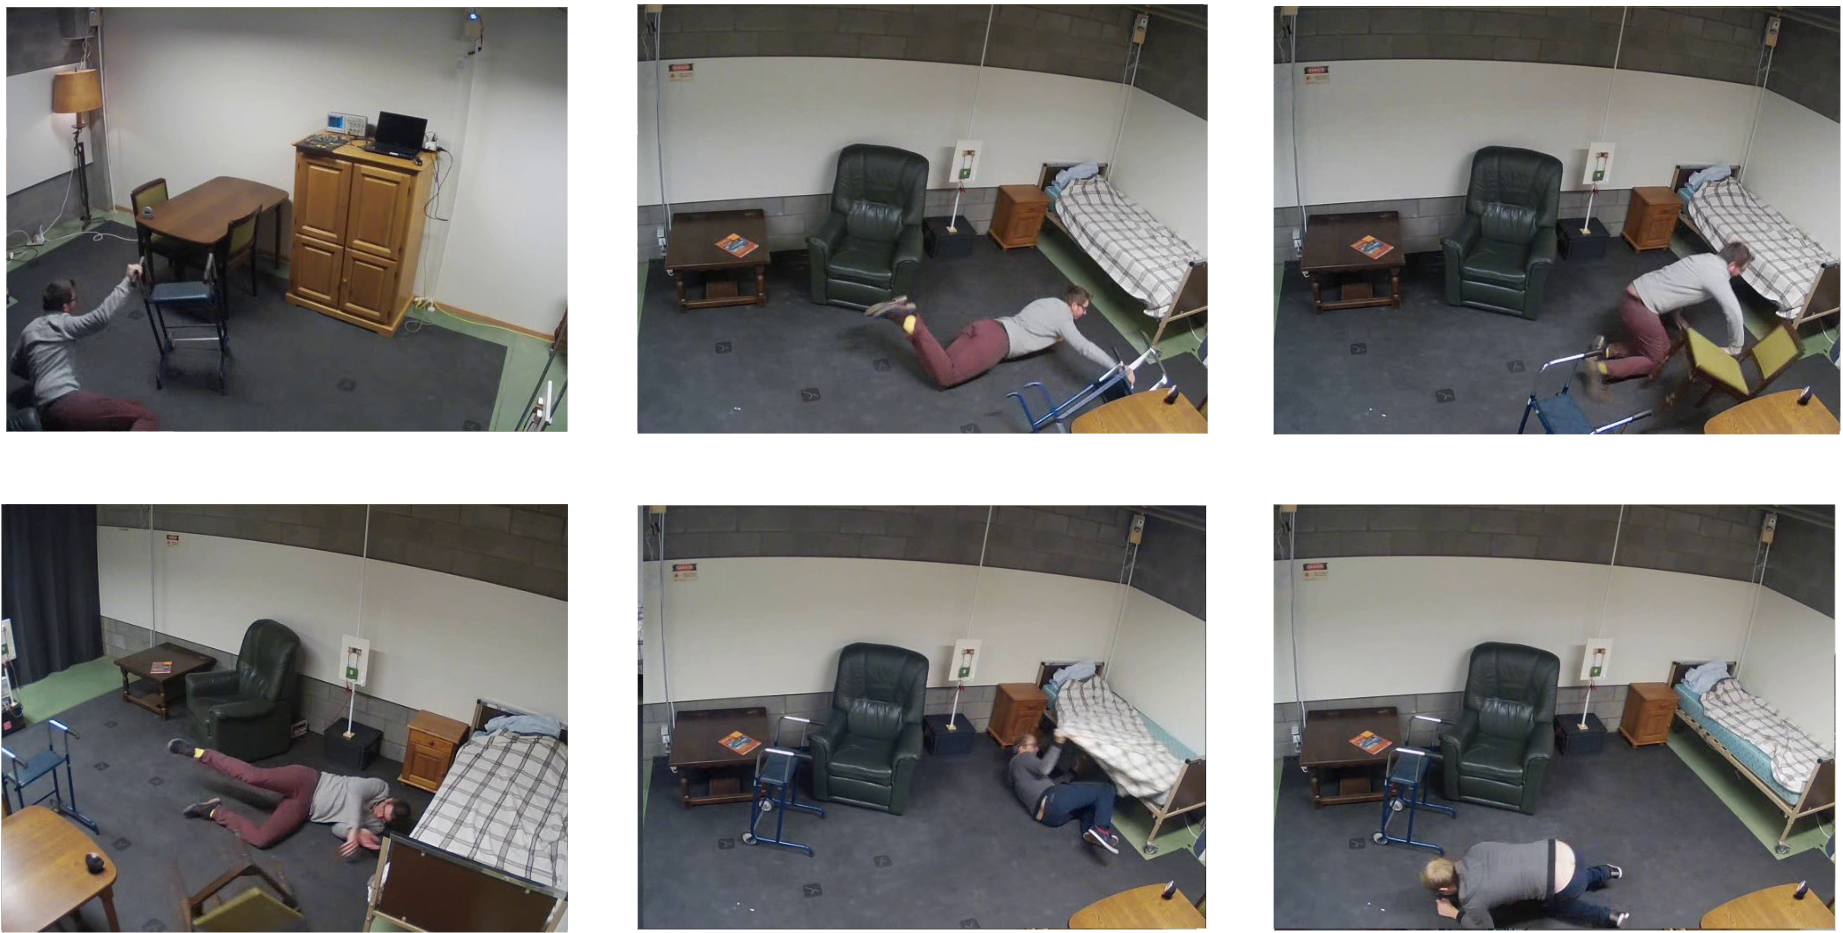
\includegraphics[width=1\textwidth]{figure/BAB 4/contoh fall.png}  % Menyisipkan gambar dengan lebar setengah lebar teks
    \caption{Contoh dataset jatuh}  % Menambahkan keterangan gambar
    \label{fig:data jatuh}  % Menambahkan label untuk referensi
\end{figure}

Dataset yang digunakan berasal dari paper \textit{“Bridging the gap between real-life data and simulated data by providing realistic fall dataset for evaluating camera-based fall detection algorithms”}, Beberapa contoh tampilan video dataset dapat dilihat pada Gambar \ref{fig:data jatuh} dan Gambar \ref{fig:data tidak jatuh}. Dataset ini berupa video gerakan tubuh yang direkam dengan kamera 2 dimensi untuk mendokumentasikan skenario jatuh dalam lingkungan realistis. Berdasarkan metadata dari Dataset ini, terdapat 270 video jatuh dan 85 video tidak jatuh. Video jatuh berdurasi 1–5 menit, sedangkan video tidak jatuh berdurasi 10–30 menit, informasi lengkapnya dapat dilihat pada Subbab \ref{III.pengumpulan data}. \par

\begin{figure}[htbp]  % 'h' menunjukkan gambar akan diletakkan di sekitar posisi ini
    \centering  % Gambar dipusatkan
    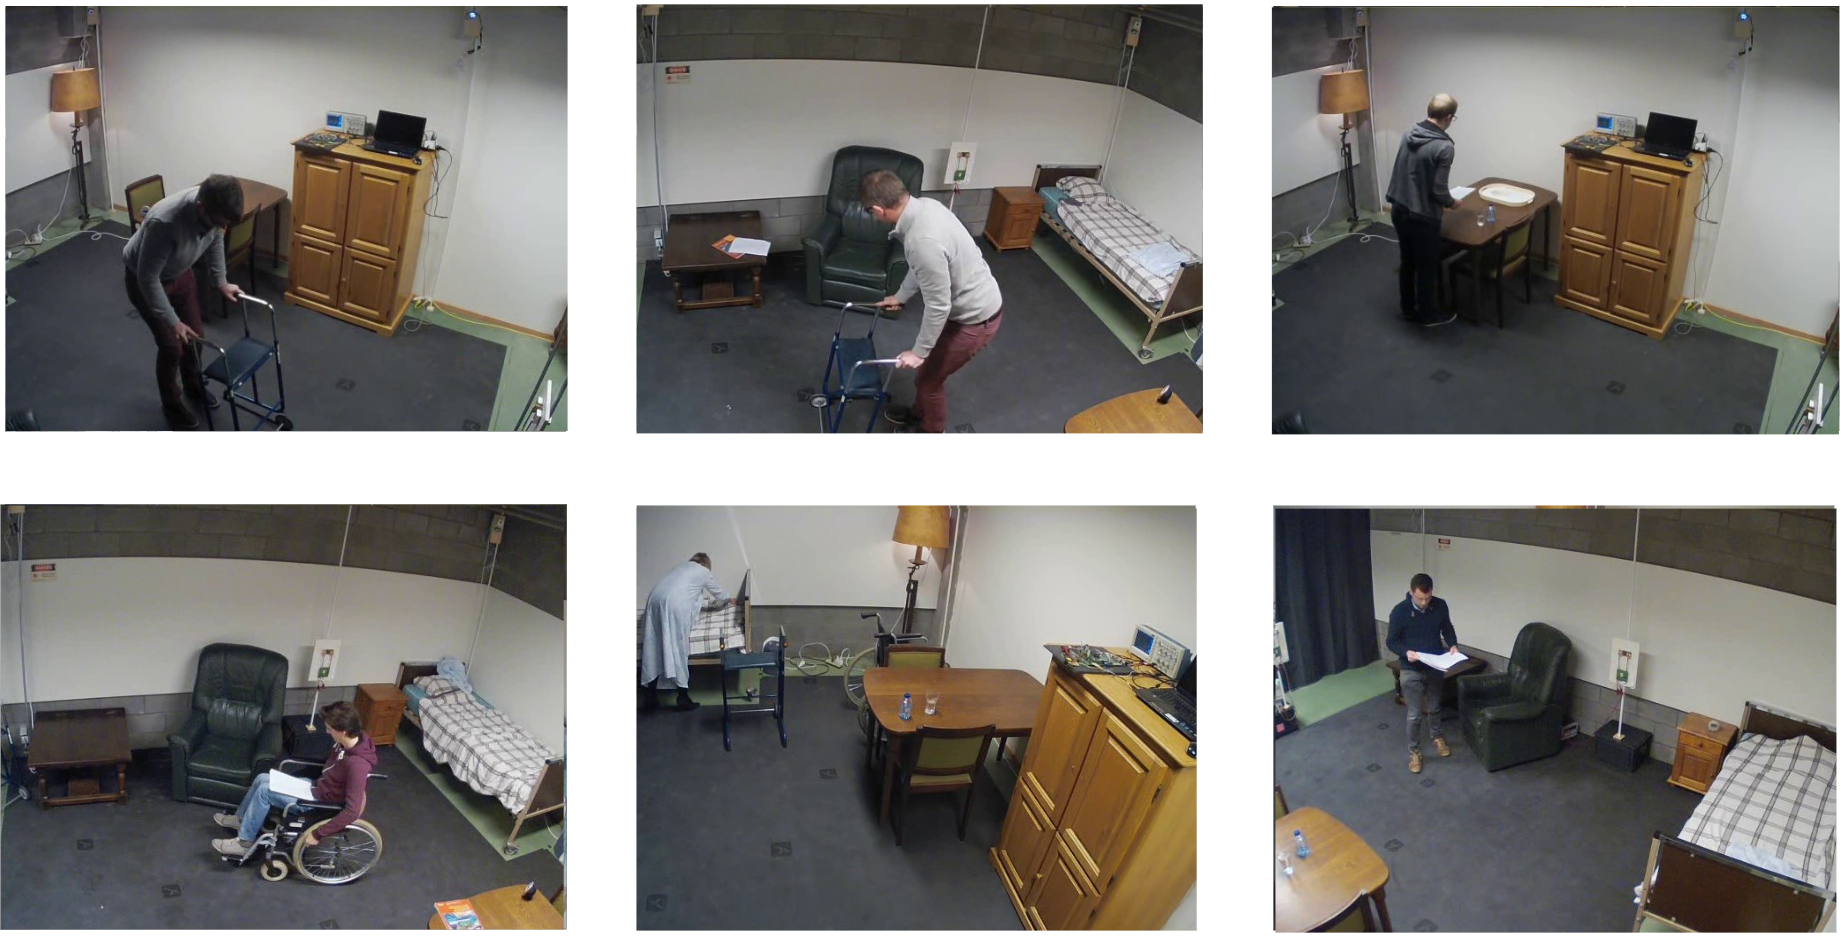
\includegraphics[width=1\textwidth]{figure/BAB 4/contoh not fall.png}  % Menyisipkan gambar dengan lebar setengah lebar teks
    \caption{Contoh dataset tidak jatuh}  % Menambahkan keterangan gambar
    \label{fig:data tidak jatuh}  % Menambahkan label untuk referensi
\end{figure}

Distribusi data pada kategori jatuh dan tidak jatuh disajikan secara lebih spesifik sesuai dengan karakteristik masing-masing video. Pada data jatuh, distribusi difokuskan pada posisi awal aktor sebelum terjadinya insiden jatuh, sehingga dapat terlihat pola awal yang memicu terjadinya jatuh. Sementara itu, pada data tidak jatuh, distribusi dihitung berdasarkan posisi aktor sepanjang durasi video untuk merepresentasikan variasi aktivitas normal yang dilakukan tanpa adanya insiden jatuh. selain itu, ternyata ada 3 video jatuh yang hilang dari dataset sehingga total data sebenarnya dari kelas jatuh sebanyak 267 video. Informasi lengkap nya dapat dilihat pada Tabel \ref{table:4.data jatuh} dan \ref{table:4.data tidak jatuh}. \par


\begin{table}[htbp]
    \centering
    \caption{Penjabaran data video jatuh}
    \label{table:4.data jatuh}
    \begin{tabular}{|c|c|c|}
        \hline
        \textbf{No} & \textbf{Posisi awal} & \textbf{Total} \\ \hline
        1 & Berdiri                    & 117 \\ \hline
        2 & Transisi berdiri--duduk   & 35  \\ \hline
        3 & Transisi duduk--berdiri   & 10  \\ \hline
        4 & Berlutut                   & 30  \\ \hline
        5 & Membungkuk                 & 25  \\ \hline
        6 & Duduk                      & 50  \\ \hline
        \multicolumn{2}{|c|}{\textbf{Total keseluruhan}} & \textbf{267} \\ \hline
    \end{tabular}
\end{table}


% Total data awal Fall: 275 
% berjalan: 21
% berdiri: 4
% transisi berdiri-duduk: 7
% transisi duduk-berdiri: 2
% on knees: 6
% bend forward: 5
% sitting: 10


\begin{table}[htbp]
    \centering
    \caption{Penjabaran data video tidak jatuh}
    \label{table:4.data tidak jatuh}
    \begin{tabular}{|c|c|c|}
        \hline
        \textbf{No} & \textbf{Posisi sepanjang video (awal--akhir)} & \textbf{Total} \\ \hline
        1 & Berdiri                  & 65 \\ \hline
        2 & Transisi berdiri--duduk  & 80 \\ \hline
        3 & Transisi duduk--berdiri  & 35 \\ \hline
        4 & Membungkuk               & 75 \\ \hline
        5 & Duduk                    & 15 \\ \hline
        \multicolumn{2}{|c|}{\textbf{Total keseluruhan}} & \textbf{270} \\ \hline
    \end{tabular}
\end{table}



% total data awal ADL: 54 (ada beberapa skenario dalam 1 durasi)
% jalan: 13
% duduk-diri: 7
% diri-duduk: 16
% diri-merunduk: 11
% duduk-merunduk: 4
% duduk (wheelchair): 3
% ganti baju: 4
% ini ada kelebihan data 4

Terlihat pada Tabel \ref{table:4.data jatuh} menyajikan rincian distribusi posisi awal aktor sebelum terjadinya insiden jatuh pada data video jatuh. Dari tabel tersebut terlihat bahwa mayoritas kejadian jatuh diawali dari posisi berdiri sebanyak 117 kali, diikuti dengan transisi berdiri–duduk sebanyak 35 kali, serta posisi duduk sebanyak 50 kali. Beberapa skenario lainnya juga melibatkan posisi berlutut (30 kali), membungkuk (25 kali), dan transisi duduk–berdiri (10 kali). Sementara itu, Tabel \ref{table:4.data tidak jatuh} menggambarkan distribusi posisi aktor sepanjang durasi video tidak jatuh yang berfungsi sebagai pembanding. Pada skenario ini, posisi yang paling dominan adalah membungkuk (75 kali) dan transisi berdiri–duduk (80 kali), kemudian diikuti oleh berdiri (65 kali), transisi duduk–berdiri (35 kali), dan duduk (15 kali).

\subsection{Prapemrosesan Dataset} \label{IV.prapemrosesan}
Pada bagian ini akan dipaparkan hasil dari proses prapemrosesan dataset. Proses tersebut menghasilkan kumpulan citra yang berhasil diekstraksi dari video, kemudian mengekstrak 33 \textit{pose landmark} manusia yang diperoleh melalui deteksi \textit{Mediapipe Pose}, disertai dengan penyamaan jumlah data antara kelas jatuh dan tidak jatuh. Selanjutnya, \textit{landmark} tersebut dikonversi menjadi bentuk graf sehingga dapat merepresentasikan hubungan spasial antar titik tubuh secara lebih terstruktur. Terakhir, membagi dataset dengan menerapakan 5-Fold untuk mencegah adanya kebocoran data dalam pelatihan model nantinya. Hasil prapemrosesan ini menjadi tahap penting karena menentukan kualitas data yang akan digunakan oleh model GCN dalam membedakan pola posisi jatuh dan tidak jatuh. \par

\subsubsection{Ekstraksi Citra Dari video} \label{IV.ekstrak frame}

Ketika program ekstraksi citra pada Kode \ref{kode:pergeseran waktu mulai} dan Kode \ref{kode:ekstrak random} dijalankan, \textit{metadata} video dibaca dari file Excel yang berisi path video, waktu mulai/akhir, dan label. Waktu dikonversi ke detik, lalu khusus kelas jatuh diterapkan \textit{adjust\_start\_sec} untuk memfokuskan rentang sampling. Terakhir, fungsi \textit{extract\_random\_frames} dipanggil untuk mengekstraksi 30 citra per video, menghasilkan dataset dengan total 537 folder yang berisi 16.110 citra siap diproses \textit{Mediapipe Pose} pada tahap berikutnya, seperti yang terlihat pada Tabel \ref{tab:total citra} \par

\begin{table}[htbp]
    \centering
    \caption{Total ekstraksi citra dari video}
    \label{tab:total citra}
    \begin{tabular}{|c|c|c|c|c|}
        \hline
        \textbf{No} & \textbf{Jenis Video} & \textbf{Total Video} & \textbf{Ekstrak Citra Video} & \textbf{Total Citra} \\ \hline
        1 & Jatuh & 267 & 30 & 8.010 \\ \hline
        2 & Tidak Jatuh & 270 & 30 & 8.100 \\ \hline
        \multicolumn{4}{|c|}{Total Citra} & 16.110 \\ \hline
    \end{tabular}
\end{table}

Tabel \ref{tab:total citra} menunjukkan proses ekstraksi citra secara ringkas. Terdapat 267 video jatuh yang masing-masing menghasilkan 30 citra, sehingga total citra yang diekstrak adalah 8.010. Sedangkan untuk video Tidak Jatuh, sebanyak 270 video juga menghasilkan 30 citra per video, dengan total citra yang diekstrak sebanyak 8.100. Secara keseluruhan, jumlah total citra yang berhasil diekstrak dari kedua jenis video adalah 16.110 citra. Citra-citra ini selanjutnya siap untuk diproses lebih lanjut pada tahap deteksi 33 \textit{pose landmark} menggunakan MediaPipe, untuk menganalisis posisi tubuh dalam setiap citra agar dapat memberikan data berupa titik-titik tubuh yang relevan. \par

\subsubsection{Deteksi 33 \textit{Pose Landmark} Dengan\textit{ MediaPipe Pose}} \label{IV.ekstrak skeleton}

Hasil \textit{pose.process} dari Kode \ref{kode:ekstrak skeleton} mengembalikan \textit{results.pose\_landmarks} yang berisi 33 titik anatomi terurut dalam bentuk koordinat ternormalisasi terhadap lebar dan tinggi citra pada rentang [0,1], dengan sumbu-x ke kanan dan sumbu-y ke bawah. normalisasi ini membuat representasi tidak bergantung pada resolusi asli dan memudahkan proyeksi ulang ke piksel saat visualisasi. Contoh \textit{preview} hasil ekstraksi pose landmark dapat dilihat pada Gambar \ref{fig:preview pose landmark}.\par

\begin{figure}[htbp]  % 'h' menunjukkan gambar akan diletakkan di sekitar posisi ini
    \centering  % Gambar dipusatkan
    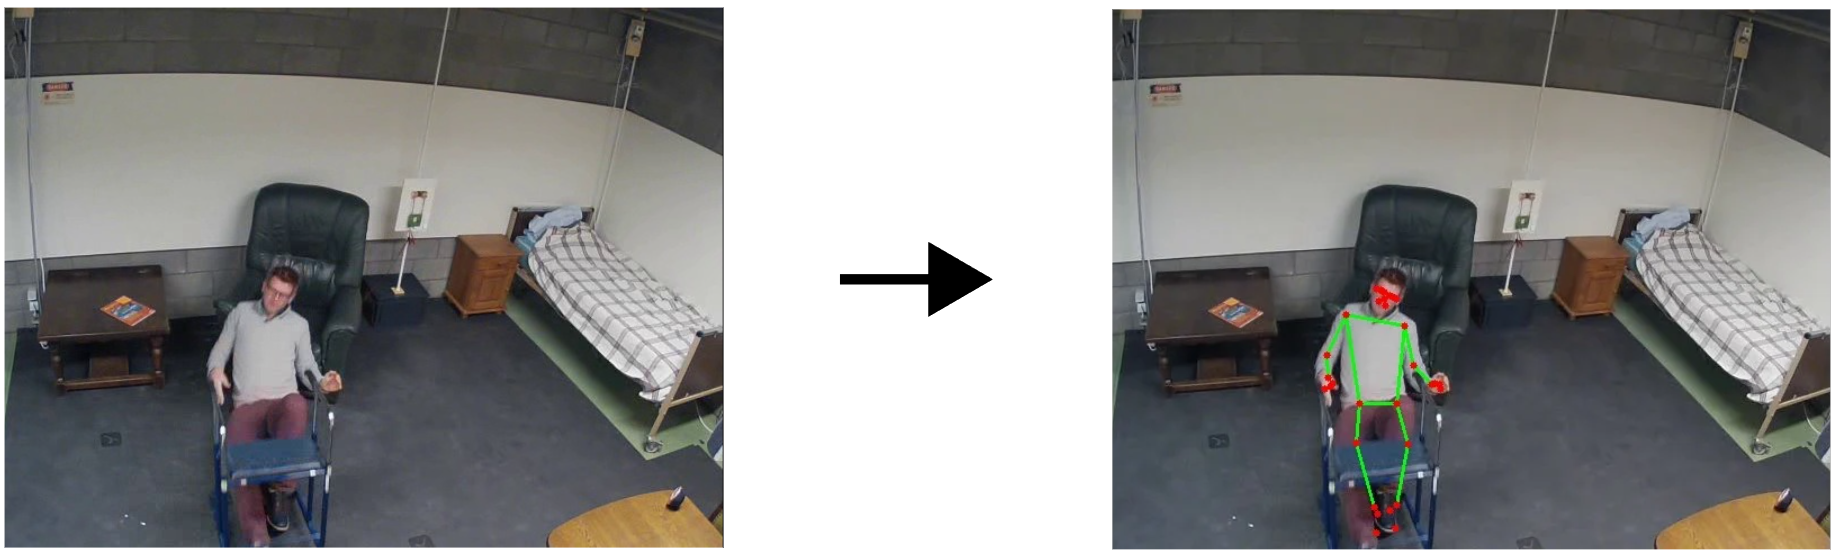
\includegraphics[width=1\textwidth]{figure/BAB 4/preview konversi citra ke pose lanmark.png}  % Menyisipkan gambar dengan lebar setengah lebar teks
    \caption{\textit{Preview} konversi citra ke \textit{pose landmark}}  % Menambahkan keterangan gambar
    \label{fig:preview pose landmark}  % Menambahkan label untuk referensi
\end{figure}

Dari seluruh citra yang diproses, terdapat 3.260 citra dengan posisi jatuh (termasuk 13 folder citra yang tidak dapat diproses) dan 3.032 citra dengan posisi tidak jatuh (termasuk 28 folder citra yang tidak dapat diproses), sehingga total citra yang gagal diproses mencapai 6.292 citra, dengan 41 folder. Hal ini disebabkan oleh hasil proses \textit{Mediapipe Pose} pada setiap citra yang memberikan tingkat keyakinan (\textit{confidence}) di bawah 0,5. Akibatnya, total dataset yang berhasil diproses oleh Mediapipe berkurang menjadi 4.750 data \textit{skeleton} untuk posisi jatuh dan 5.068 data \textit{skeleton} untuk posisi tidak jatuh. Demi mengantisipasi kesenjangan jumlah data antara kedua kelas, dilakukan penghapusan data secara acak pada kelas tidak jatuh agar memiliki jumlah yang sama dengan kelas jatuh, rinciannya dapat dilihat pada Tabel \ref{tab:total skeleton} \par

\begin{table}[htbp]
    \centering
    \caption{Total ekstraksi skeleton dari citra}
    \label{tab:total skeleton}
    \begin{tabular}{|c|c|c|c|c|c|}
        \hline
        \multirow{2}{*}{\textbf{No}} & \multirow{2}{*}{\textbf{Jenis Citra}} & \multirow{2}{*}{\textbf{Total Citra}} & \multicolumn{3}{c|}{\textbf{Jumlah Ekstraksi Skeleton}} \\ \cline{4-6}
        & & & \textbf{Berhasil} & \textbf{Gagal} & \textbf{penyamaan} \\ \hline
        1 & Jatuh & 8.010 & 4.750 & 3.260 & 4.750 \\ \hline
        2 & Tidak Jatuh & 8.100 & 5.068 & 3.032 & 4.750 \\ \hline
        \multicolumn{5}{|c|}{Total keseluruhan} & 9.500 \\ \hline
    \end{tabular}
\end{table}

Berdasakan perbedaan jumlah antara kedua kelas tersebut, dilakukan penghapusan data secara acak pada data \textit{skeleton} dengan posisi tidak jatuh hingga jumlahnya setara dengan data \textit{skeleton} posisi jatuh. Sehingga, total data \textit{skeleton} yang tersedia menjadi 9.500 (499 folder), dengan masing-masing kelas berjumlah 4.750 data. Contoh citra yang tidak dapat diproses dapat dilihat pada Gambar \ref{fig:contoh citra gagal diproses mediapipe}. Pada citra-citra tersebut, sebagian tubuh terpotong sehingga menghambat proses \textit{Mediapipe Pose} dan menghasilkan tingkat keyakinan di bawah 0,5, sehingga data \textit{skeleton} dari citra tersebut tidak disimpan. \par

\begin{figure}[htbp]  % 'h' menunjukkan gambar akan diletakkan di sekitar posisi ini
    \centering  % Gambar dipusatkan
    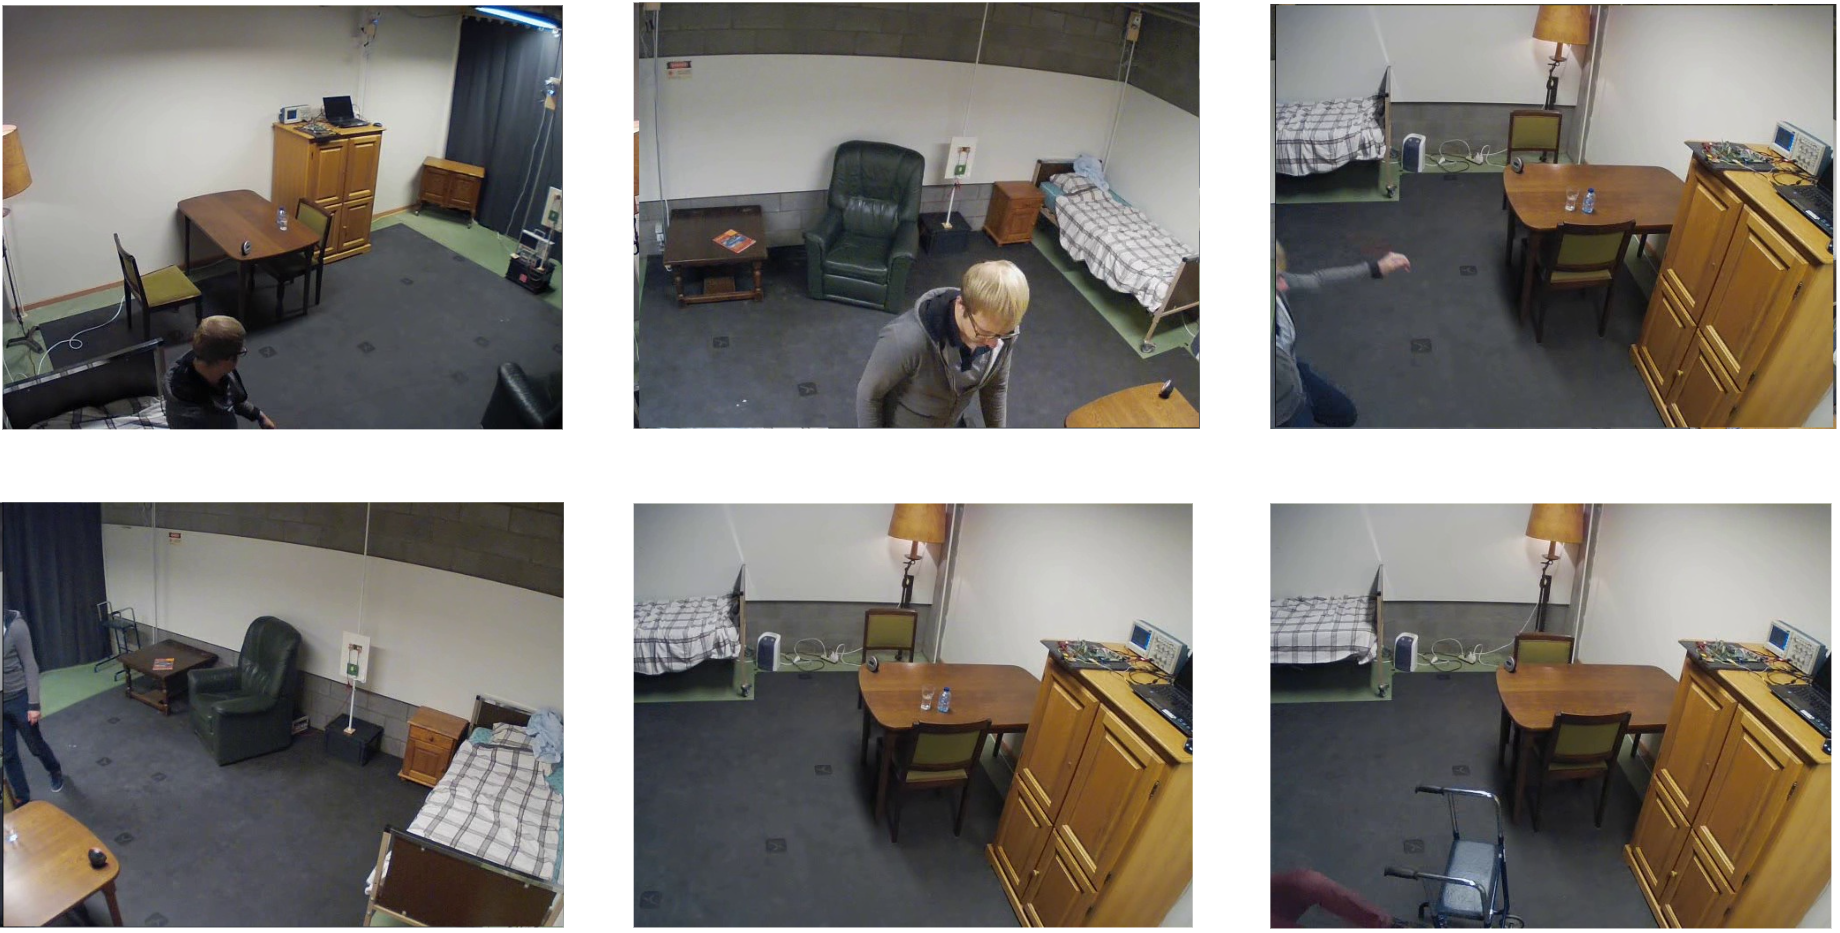
\includegraphics[width=1\textwidth]{figure/BAB 4/contoh citra gagal diproses mediapipe.png}  % Menyisipkan gambar dengan lebar setengah lebar teks
    \caption{Contoh citra gagal diproses \textit{Mediapipe Pose}}  % Menambahkan keterangan gambar
    \label{fig:contoh citra gagal diproses mediapipe}  % Menambahkan label untuk referensi
\end{figure}

\subsubsection{Konversi \textit{Pose Landmark} Ke Graf} \label{IV.konversi graf}

\begin{figure}[htbp]  % 'h' menunjukkan gambar akan diletakkan di sekitar posisi ini
    \centering  % Gambar dipusatkan
    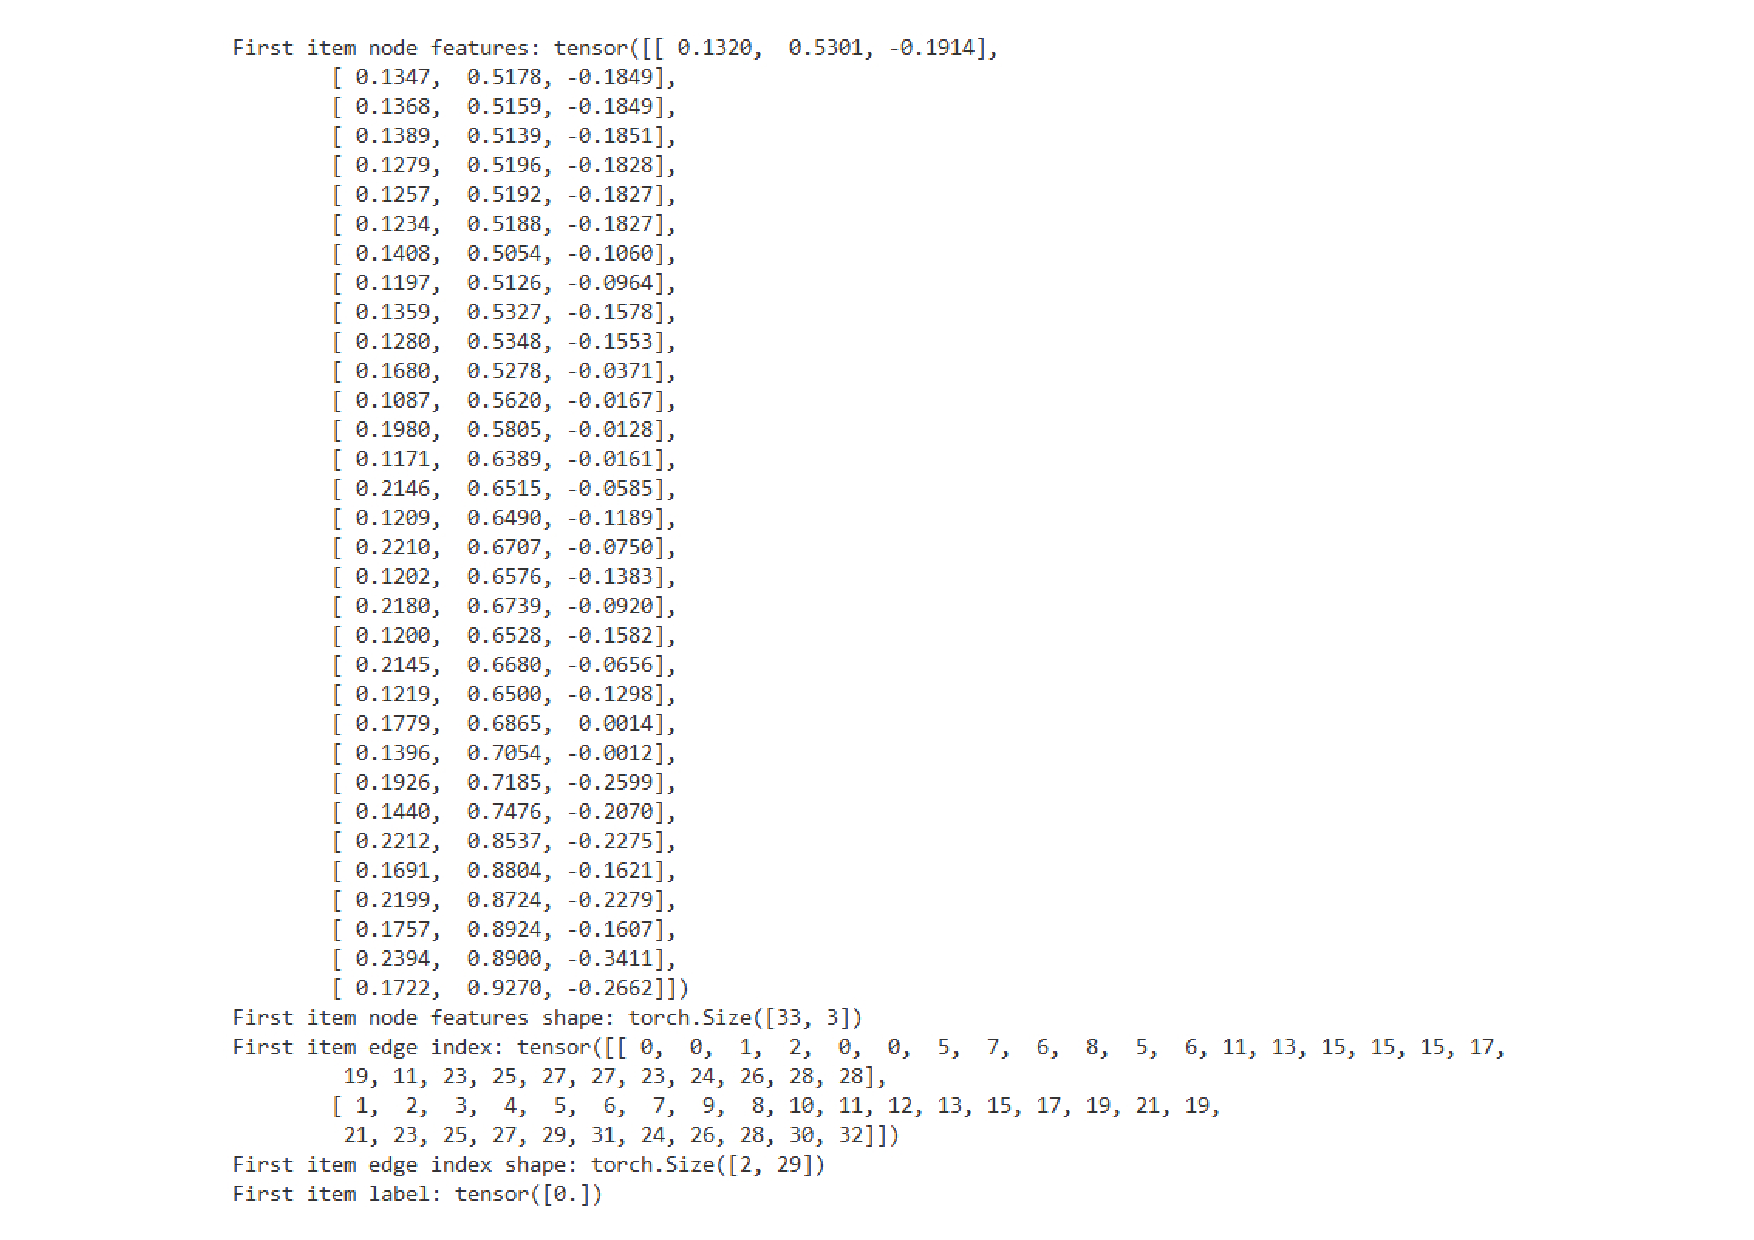
\includegraphics[width=1\textwidth]{figure/BAB 3/contoh data graf.pdf} 
    \caption{Contoh tampilan data graf.}  % Menambahkan keterangan gambar
    \label{fig:contoh data graf}  % Menambahkan label untuk referensi
\end{figure}

Ketika menjalankan rancangan Kode \ref{kode:skeleton edges} dan Kode \ref{kode:konversi skeleton graf}, informasi yang ditampilkan pada Gambar \ref{fig:contoh data graf} menunjukkan data graf yang berasal dari konversi data skeleton menjadi format graf. Data graf ini terdiri dari beberapa komponen utama. Pertama, terdapat \textit{node features}, menjabarkan atribut atau fitur yang dimiliki oleh setiap node dalam graf. Setiap node memiliki tiga fitur yang tercatat dalam format tensor, yang bisa merepresentasikan koordinat dari node tersebut. \par

Selanjutnya, edge index yang menggambarkan hubungan antara node-node dalam graf. Setiap edge menghubungkan dua node dan diindeks dengan pasangan angka, di mana setiap pasangan menunjukkan node sumber dan node tujuan. Jumlah edge yang ada adalah 29, yang mengindikasikan adanya 29 hubungan antar node. Edge index shape memberikan informasi tentang dimensi data edge tersebut, yang menunjukkan bahwa ada dua baris data (untuk node sumber dan tujuan) dan 29 kolom (untuk jumlah edge). Terakhir, terdapat label sebagai identitas keseluruhan data tersebut dalam bentuk nilai tensor, sehingga semua komponen ini membentuk struktur data graf yang lengkap, dan siap digunakan untuk pelatihan model klasifikasi jatuh dan tidak jatuh pada lansia. \par



% \begin{figure}[H]  % 'h' menunjukkan gambar akan diletakkan di sekitar posisi ini
%     \centering  % Gambar dipusatkan
%     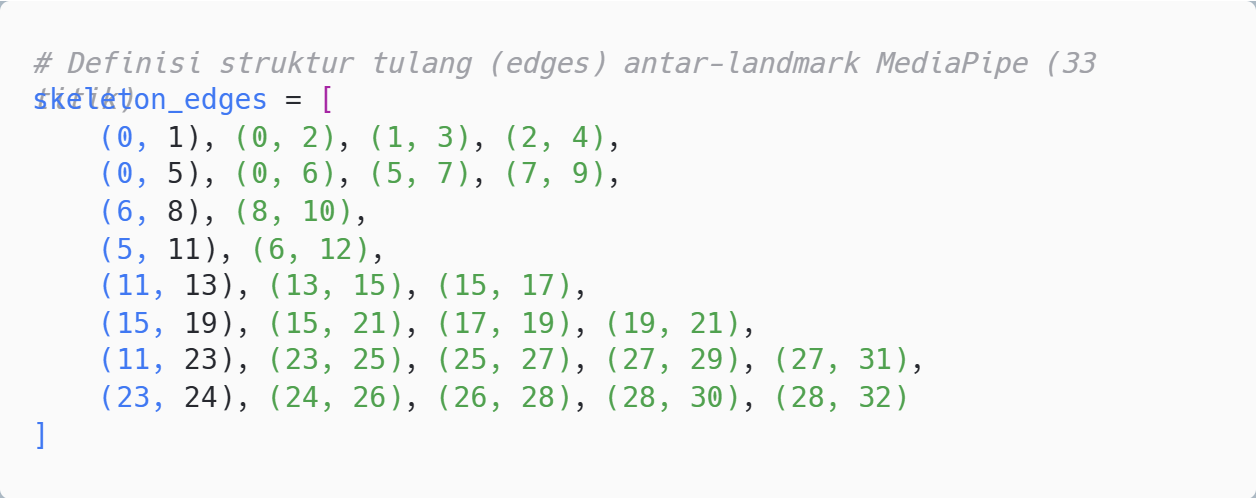
\includegraphics[width=1\textwidth]{images/skeleton_edges.png}  % Menyisipkan gambar dengan lebar setengah lebar teks
%     \label{fig:kode skeleton edges}  % Menambahkan label untuk referensi
% \end{figure}
% Pada Gambar \ref{fig:kode skeleton edges} terlihat Daftar \textit{skeleton\_edges} yang mendefinisikan graf kerangka berdasarkan indeks \textit{landmark MediaPipe} (0–32). Tiap pasangan (u, v) menyatakan sisi terarah (yang kemudian ditranspos menjadi bentuk [2, E] untuk PyG) antara dua sendi, mencakup koneksi utama tubuh atas (mata, bahu, siku, pergelangan) hingga tubuh bawah (pinggul, lutut, pergelangan kaki, tumit, ujung kaki). Daftar ini menyandikan pengetahuan anatomi ke dalam struktur graf sehingga GCN dapat mengeksploitasi kedekatan struktural antartitik. \par

% \begin{figure}[H]  % 'h' menunjukkan gambar akan diletakkan di sekitar posisi ini
%     \centering  % Gambar dipusatkan
%     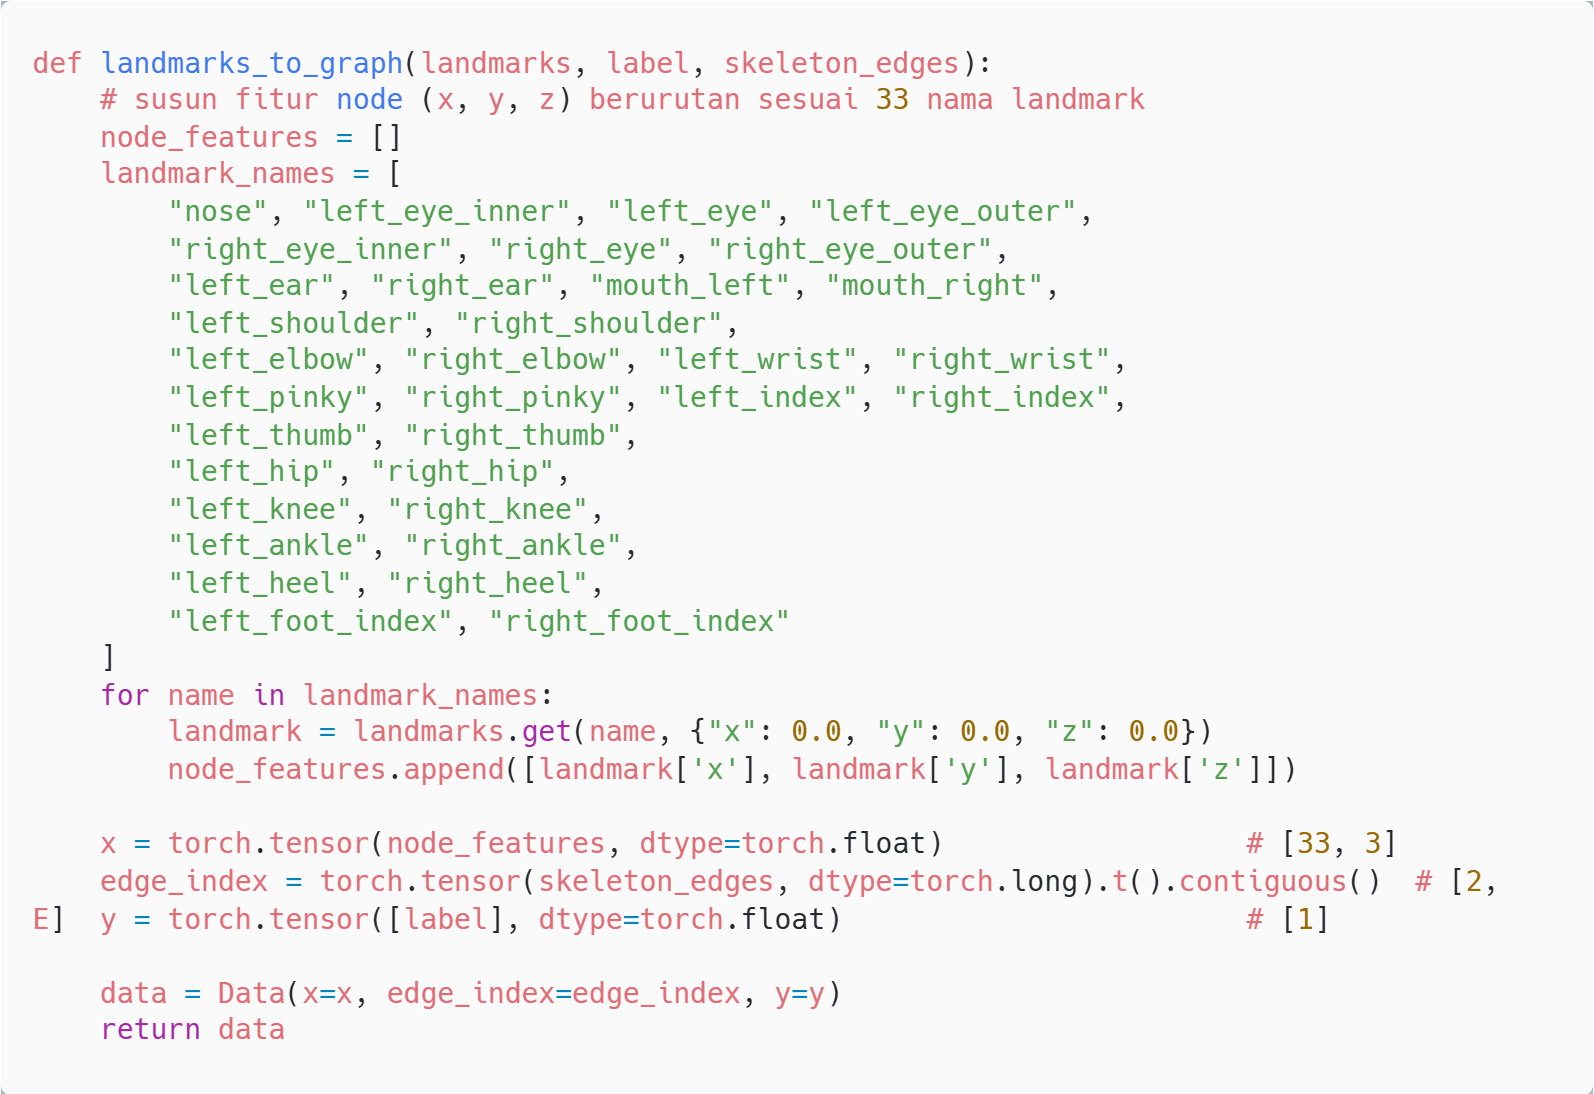
\includegraphics[width=1\textwidth]{images/landmark_to_graph.png}  % Menyisipkan gambar dengan lebar setengah lebar teks
%     \caption{Kode konversi \textit{skeleton} ke graf}  % Menambahkan keterangan gambar
%     \label{fig:kode konversi skeleton graf}  % Menambahkan label untuk referensi
% \end{figure}

% Fungsi \textit{landmarks\_to\_graph} pada Gambar \ref{fig:kode konversi skeleton graf} mengubah hasil deteksi pose menjadi graf \textit{PyTorch Geometric} (torch\_geometric.data.Data) yang siap untuk pelatihan GCN. Pertama, urutan \textit{landmark\_names} menegakkan indeks node yang konsisten (0–32), sehingga setiap sampel selalu menyusun fitur node [x, y, z] dalam urutan identik. Ini penting agar filter konvolusi graf melihat node yang sama di posisi yang sama antar-sampel. Tensor x berukuran [33, 3] memuat fitur koordinat 3 dimensi, sedangkan \textit{edge\_index} adalah indeks sisi [2, E] hasil \textit{t().contiguous()} agar kompatibel dengan kernel PyG. Label y dibuat sebagai tensor (1) bertipe float—konvensi umum untuk klasifikasi biner.



\subsubsection{Pembagian K-Fold Pada Dataset} \label{IV.K-Fold}

\begin{table}[H]
    \centering
    \caption{Hasil penbagian E-Fold pada dataset per folder }
    \label{tab:data k-fold}
    \begin{tabular}{|c|c|c|c|c|c|c|c|}
        \hline
        \multirow{2}{*}{\textbf{Iterasi}} & \multicolumn{5}{c|}{\textbf{K-Fold per Folder}} & \multirow{2}{*}{\textbf{Data Train}} & \multirow{2}{*}{\textbf{Data Validation}} \\ \cline{2-6}
         & \textbf{1} & \textbf{2} & \textbf{3} & \textbf{4} & \textbf{5} & & \\ \hline 
        1 & \cellcolor{yellow}100 & 100 & 100 & 100 & 99 & 6,969 & 2,531 \\ \hline
        2 & 100 & \cellcolor{yellow}100 & 100 & 100 & 99 & 8,151 & 1,349 \\ \hline
        3 & 100 & 100 & \cellcolor{yellow}100 & 100 & 99 & 7,159 & 2,341 \\ \hline
        4 & 100 & 100 & 100 & \cellcolor{yellow}100 & 99 & 7,922 & 1,578 \\ \hline
        5 & 100 & 100 & 100 & 100 & \cellcolor{yellow}99 & 7,799 & 1,701 \\ \hline
        \multicolumn{6}{|c|}{Total Keseluruhan} & \multicolumn{2}{c|}{9,500}\\ \hline
    \end{tabular}
\end{table}

Pada Tabel \ref{tab:data k-fold} ditunjukkan skema hasil pembagian data 5-fold berbasis folder (bukan per file) yang didapatkan setelah menjalankan Kode \ref{kode:generate k-fold} untuk mencegah kebocoran data antar set. Pada tiap iterasi (1–5), satu kelompok folder dijadikan validasi (sel berwarna), sementara empat kelompok lainnya dipakai untuk pelatihan. Total terdapat 499 folder pada dataset, sehingga dibagi menjadi 5 kelompok, empat kelompok berisi 100 folder dan satu kelompok berisi 99 folder—itulah sebabnya kolom “K-Fold per Folder” berisi angka 100 dan 99. Meski jumlah folder per kelompok tetap, kolom \textit{Data Train} dan \textit{Data Validation} dapat bervariasi antar iterasi karena tiap folder menyimpan jumlah file yang berbeda. Dengan rancangan ini, dipastikan tidak ada konten dari folder yang sama muncul di train dan validasi secara bersamaan. \par


\subsection{Perancangan Model Klasifikasi} \label{IV.Perancangan}

 Pada Kode \ref{kode:inisialisasi gcn} dipaparkan inisialisasi komponen membangun arsitektur GCN. Setiap lapis konvolusi graf (GCNConv) diikuti batch normalization (BatchNorm1d) untuk menstabilkan distribusi aktivasi pada domain graf. Mekanisme dropout disiapkan untuk regularisasi, sementara bagian klasifikasi menggunakan MLP dua lapis (final\_lin1 dan final\_lin2) berfungsi memetakan \textit{embedding global} ke ruang kelas. Pemilihan fungsi \textit{global pooling} bersifat parametrik (mean, max, atau add) untuk mereduksi representasi tingkat-node menjadi vektor tingkat-graf, sehingga model dapat menyesuaikan dengan karakteristik data. Penyelarasan seed pada awal konstruktor menjaga konsistensi inisialisasi bobot selama eksperimen. \par

Fungsi \textit{forward} pada Kode \ref{kode:inisialisasi gcn} merealisasikan alur inferensi dari tingkat-node hingga prediksi kelas. Setiap blok konvolusi graf menggabungkan penyebaran informasi topologis melalui \textit{GCNConv}, normalisasi aktivasi dengan \textit{BatchNorm1d}, fungsi aktivasi nonlinier ReLU, dan dropout untuk mengurangi \textit{overfitting}. Opsi \textit{residual connection} diaktifkan secara kondisional ketika dimensi fitur kompatibel, sehingga gradien dapat mengalir lebih stabil pada jaringan yang lebih dalam dan mengurangi degradasi representasi. Setelah tumpukan konvolusi, \textit{global pool} mengagregasi fitur node menjadi embedding graf berbasis vektor batch (yang menandai keanggotaan setiap node di graf \textit{mini-batch}). Kepala MLP kemudian memproyeksikan embedding global ke ruang output. Aktivasi keluaran \textit{sigmoid} untuk klasifikasi biner dengan satu neuron keluaran. \par

\section{Evaluasi Hasil} \label{IV.evaluasi}
Pada subbab ini akan dijelaskan secara rinci bagaimana hasil pelatihan model menggunakan konfigurasi hyperparameter default dan konfigurasi hyperparameter studi ablasi. \par

\subsection{Evaluasi Model dengan \textit{Hyperparameter Default}} \label{IV.evaluasi-default}

\begin{table}[htbp]
    \centering
    \caption{Konfigurasi \textit{hyperparameter} untuk pelatihan model GCN}
    \label{tab:hyperparams-gcn}
    \begin{tabular}{|c|l|l|}
        \hline
        \textbf{No} & \textbf{\textit{Hyperparameter}} & \textbf{Nilai} \\ \hline
        1 & \textit{optimizers}          & AdamW \\ \hline
        2 & \textit{learning\_rates}     & 1e-3 \\ \hline
        3 & \textit{weight\_decays}      & 1e-5 \\ \hline
        4 & \textit{batch\_sizes}        & 32 \\ \hline
        5 & \textit{dropout\_rates}      & 0.3 \\ \hline
        6 & \textit{epochs}              & 100 \\ \hline
        7 & \textit{hidden\_channels}    & [64, 32, 32, 32, 32] \\ \hline
        8 & \textit{residuals}           & \textit{True} \\ \hline
    \end{tabular}
\end{table}


Berbagai nilai \textit{Hyperparameter} pada Tabel \ref{tab:hyperparams-gcn} memperlihatkan pengaturan dasar yang digunakan pada seluruh eksperimen. Pelatihan dijalankan selama 100 epoch dengan ukuran batch 32. Skema optimisasi menggunakan AdamW dengan laju belajar \(1\times 10^{-3}\) dan weight decay \(1\times 10^{-5}\), yang menjaga stabilitas pembaruan bobot sekaligus membantu menekan \textit{overfitting}. Arsitektur GCN menerima 3 fitur per node (\(x,y,z\)) dan menggunakan tumpukan hidden channels \([64, 32, 32, 32, 32]\) yang dipadukan dengan dropout 0,3 sebagai regularisasi. Residual connection diaktifkan agar aliran gradien tetap stabil pada jaringan yang lebih dalam. Secara keseluruhan, konfigurasi ini merupakan kompromi yang baik: cukup ekspresif untuk mempelajari relasi spasial antartitik pose, namun tetap terkontrol dari sisi kompleksitas dan risiko \textit{overfitting}. \par

% \begin{table}[htbp]
% \centering
% \caption{Hasil evaluasi per fold dan rerata}
% \label{tab:evaluasi-fold}
% \begin{tabular}{ccccccccc}
% \toprule
% \multirow{2}{*}{\textbf{fold}} &
% \multicolumn{4}{c}{\textbf{hasil \textit{confusion matrix}}} &
% \multicolumn{4}{c}{\textbf{metrik evaluasi}} \\
% \cmidrule(lr){2-5}\cmidrule(lr){6-9}
%  & \textbf{TP} & \textbf{TN} & \textbf{FP} & \textbf{FN} & \textbf{acc} & \textbf{pre} & \textbf{rec} & \textbf{f1} \\
% \midrule
% 1 & 1105 & 558 & 592 & 276 & 0.6571 & 0.6964 & 0.6571 & 0.6668 \\
% 2 & 232 & 613 & 43 & 461 & 0.6264 & 0.8122 & 0.6264 & 0.6619 \\
% 3 & 1165 & 425 & 299 & 452 & 0.6792 & 0.6705 & 0.6792 & 0.6718 \\
% 4 & 419 & 703 & 138 & 318 & 0.7110 & 0.7415 & 0.7110 & 0.7172 \\
% 5 & 594 & 501 & 163 & 443 & 0.6437 & 0.6737 & 0.6437 & 0.6405 \\
% \midrule
% \textit{Rata-rata} &  &  &  &  & 0.6647 & 0.6939 & 0.5895 & 0.6375 \\
% \bottomrule
% \end{tabular}
% \end{table}

\begin{table}[htbp]
    \centering
    \caption{Hasil evaluasi konfigurasi default per fold dan rerata}
    \label{tab:evaluasi-fold}
    \begin{tabular}{|c|c|c|c|c|c|c|c|c|}
        \hline
        \multirow{2}{*}{\textbf{Fold}} & \multicolumn{4}{c|}{\textbf{Hasil \textit{Confusion Matrix}}} & \multicolumn{4}{c|}{\textbf{Metrik Evaluasi}} \\ \cline{2-9}
         & \textbf{TP} & \textbf{TN} & \textbf{FP} & \textbf{FN} & \textbf{Acc} & \textbf{Pre} & \textbf{Rec} & \textbf{F1} \\ \hline
        1 & 558 & 1105 & 592 & 276 & 0,657 & 0,696 & 0,657 & 0,667 \\ \hline
        2 & 613 & 232 & 43 & 461 & 0,626 & \textbf{0,812} & 0,626 & 0,662 \\ \hline
        3 & 425 & 1165 & 299 & 452 & 0,679 & 0,671 & 0,679 & 0,672 \\ \hline
        4 & 703 & 419 & 138 & 318 & \textbf{0,711} & 0,742 & \textbf{0,711} & \textbf{0,717} \\ \hline
        5 & 501 & 594 & 163 & 443 & 0,644 & 0,674 & 0,644 & 0,641 \\ \hline
        \multicolumn{5}{|c|}{\textit{Rata-rata}} & 0,665 & 0,694 & 0,59 & 0,638 \\ \hline
    \end{tabular}
\end{table}


Tabel \ref{tab:evaluasi-fold} menampilkan ringkasan confusion matrix dan metrik evaluasi utama untuk setiap \textit{fold}. Kinerja model bervariasi dengan akurasi berkisar antara 0,644 hingga 0,711, dengan rerata 0,665. Rata-rata precision lebih tinggi (0,694) dibanding recall (0,590), yang mengarah pada F1-score rata-rata 0,638. Pola ini mengindikasikan bahwa model cenderung lebih fokus untuk meminimalkan false positives (FP) daripada menangkap semua kejadian positive (FN). Sebagai contoh, pada Fold 2, meskipun precision mencapai 0,812 berkat rendahnya FP (43), recall dan akurasi lebih rendah (0,626) karena banyak FN (461) yang menunjukkan bahwa model gagal mendeteksi sebagian besar kejadian jatuh. Sebaliknya, Fold 4 memberikan keseimbangan terbaik antara precision dan recall, dengan TP = 703, FN = 318, FP = 138, dan TN = 419, menghasilkan akurasi = 0,711 dan F1 = 0,717, yang menunjukkan bahwa fold ini memberikan hasil paling optimal dalam hal deteksi posisi jatuh. Variasi antara fold ini dapat dijelaskan oleh perbedaan distribusi kasus dalam setiap fold, yang mencerminkan pembagian data yang tidak selalu seimbang dalam kelompok K-Fold. Secara keseluruhan, model menunjukkan kecenderungan untuk menghindari false alarm (tinggi precision), meskipun dengan konsekuensi recall yang sedikit lebih rendah. \par

\begin{figure}[H]  % 'h' menunjukkan gambar akan diletakkan di sekitar posisi ini
    \centering  % Gambar dipusatkan
    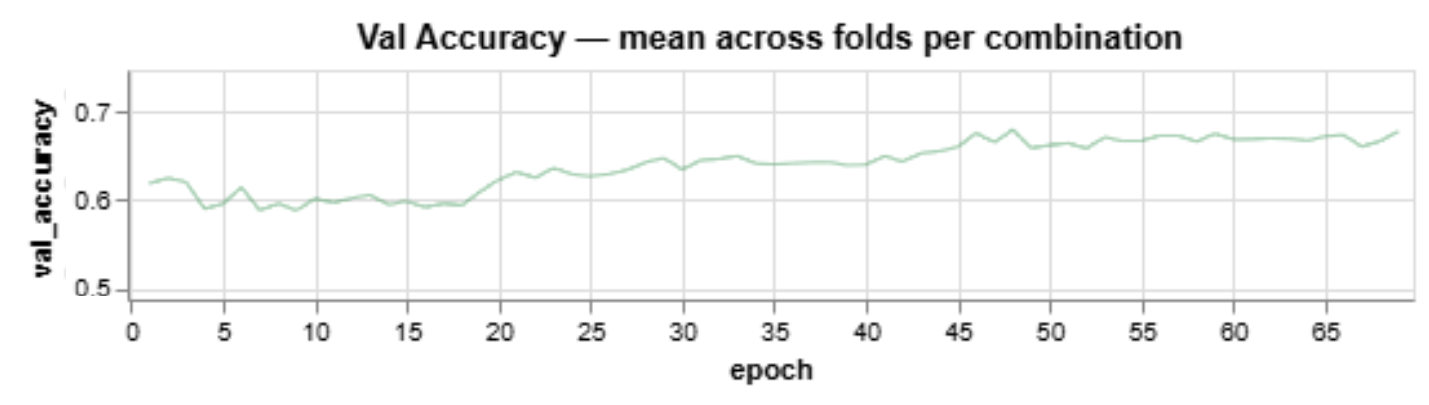
\includegraphics[width=1\textwidth]{images/akurasi model hyperparameter default.png}  % Menyisipkan gambar dengan lebar setengah lebar teks
    \caption{akurasi hasil pelatihan model GCN dengan hyperparameter default}  % Menambahkan keterangan gambar
    \label{fig:tren akurasi pelatihan default}  % Menambahkan label untuk referensi
\end{figure}

Kurva pada Gambar \ref{fig:tren akurasi pelatihan default} menunjukkan rata-rata akurasi validasi lintas lima fold pada setiap epoch. Terlihat pola peningkatan yang relatif stabil dari kisaran awal \(\approx 0{,}60{-}0{,}62\) menuju \(\approx 0{,}68{-}0{,}69\) pada akhir pelatihan. Setelah fluktuasi kecil di awal, kurva cenderung \textit{converge} secara bertahap mulai sekitar \(\sim\)epoch 35–40, lalu berfluktuasi tipis dengan tren naik hingga akhir. Tidak tampak indikasi kuat \textit{overfitting} pada data validasi (tidak ada penurunan sistematis menjelang akhir), sehingga kombinasi \emph{AdamW + learning rate} \(1\times 10^{-3}\) + \emph{dropout} 0{,}3 + \emph{residual} dapat dinilai stabil pada konfigurasi ini. Dari sisi efisiensi, karena kenaikan setelah \(\sim\)epoch 50 relatif marginal, \textit{early stopping} berbasis \textit{patience} sebanyak 10 berpotensi memangkas waktu pelatihan tanpa mengorbankan kinerja. Secara keseluruhan, kurva ini mengonfirmasi temuan pada tabel: performa validasi konsisten pada kisaran \(0{,}66{-}0{,}69\) selaras dengan rerata akurasi 5-Fold (0.6647), serta menegaskan stabilitas pembelajaran model pada pengaturan hyperparameter default. \par


\subsection{Uji Model Terbaik Pada Data Primer} \label{IV.testing}
Pada penelitian ini, evaluasi model dilakukan dengan menggunakan bobot terbaik yang diperoleh berdasarkan akurasi hasil pelatihan model pada fold 4, epoch ke-2, yang menghasilkan akurasi validasi sebesar 0.71. Bobot tersebut kemudian digunakan untuk mengevaluasi kinerja model dengan hyperparameter default menggunakan dataset primer. Evaluasi akurasi model mencakup penjabaran metrix evaluasi serta pemaparan hasil prediksi terhadap setiap Citra dalam dataset primer. \par

\begin{figure}[H]  % 'h' menunjukkan gambar akan diletakkan di sekitar posisi ini
    \centering  % Gambar dipusatkan
    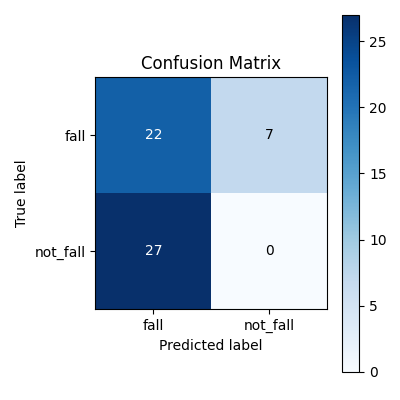
\includegraphics[width=0.45\textwidth]{figure/BAB 4/testing_confusion_matrix.png}  % Menyisipkan gambar dengan lebar setengah lebar teks
    \caption{Confusion matrix data test}  % Menambahkan keterangan gambar
    \label{fig:cm testing}  % Menambahkan label untuk referensi
\end{figure}

Pada Gambar \ref{fig:cm testing} terlihat bahwa hasil testing model klasifikasi posisi jatuh dan tidak jatuh pada data primer, model dapat memberikan prediksi yang tepat pada 22 gambar dengan label jatuh. Namun model tetap cenderung melakukan kesalahan prediksi ke arah "jatuh" pada data dengan label "tidak jatuh". \par

\begin{table}[htbp]
\centering
\caption{Hasil evaluasi testing}
\label{tab:evaluasi-testing}
\begin{tabular}{|c|c|c|c|c|c|c|c|}
\hline
\multicolumn{4}{|c|}{\textbf{Hasil \textit{confusion matrix}}} &
\multicolumn{4}{c|}{\textbf{Metrik evaluasi}} \\
\hline
\textbf{TP} & \textbf{TN} & \textbf{FP} & \textbf{FN} &
\textbf{acc} & \textbf{pre} & \textbf{rec} & \textbf{f1} \\
\hline
22 & 0 & 27 & 7 & 0,39 & 0,45 & 0,76 & 0,56 \\
\hline
\end{tabular}
\end{table}

Metrik evaluasi model pada \textit{data testing} dapat dilihat pada Tabel \ref{tab:evaluasi-testing}. Hasil metrik model dalam memprediksi data \textit{test} ternyata kurang memuaskan.Terlihat kesalahan prediksi yang berat pada 1 kelas yaitu kelas jatuh memberikan nilai akurasi sebesar 0,39. Rendahnya performa ini disebabkan oleh pengambilan data uji kelas tidak jatuh yang berasal dari video aktivitas duduk di kursi. Meskipun dataset mentah untuk pelatihan model mencakup 115 video transisi berdiri-duduk dan duduk-berdiri atau sebanyak $155 x 30 = 3.450$ citra, terdapat kemungkinan bahwa tahapan prapemrosesan seperti ekstraksi skeleton dari citra menggunakan \textit{mediapipe pose} dengan threshold 0,5 menyebabkan pengurangan data pada kelas tidak jatuh. Hal tersebut mengakibatkan adanya \textit{imbalanced} data antara kelas jatuh dengan kelas tidak jatuh. \par

Berdasarkan hal ini, dilakukan penyamaan jumlah data kelas jatuh dapat mengurangi representasi kejadian transisi duduk tersebut. Ditambah lagi Selain itu, kemiripan postur pada kejadian jatuh dengan transisi duduk menyebabkan model kesulitan untuk membedakan kejadian antara kelas jatuh dan tidak jatuh, terutama pada transisi berdiri-duduk ataupun duduk-berdiri. Ditampilkan sebagian hasil prediksi data test menggunakan model yang telah dilatih sebelumnya pada tabel \ref{tab:prediksi_model}. \par

\begin{longtable}{| c | >{\centering\arraybackslash}p{0.35\textwidth} | >{\centering\arraybackslash}p{0.2\textwidth} | >{\centering\arraybackslash}p{0.2\textwidth} |}
    \caption{Hasil Prediksi Model Akhir} \label{tab:prediksi_model} \\ 
    \hline
    \textbf{No} & \textbf{Citra Input} & \textbf{Hasil Prediksi} & \textbf{Label Aktual} \\
    \hline
    \endfirsthead

    \hline
    \textbf{No} & \textbf{Citra Input} & \textbf{Hasil Prediksi} & \textbf{Label Aktual} \\
    \hline
    \endhead

    \hline
    \endfoot

    \hline
    \endlastfoot

    % ----- Row 1 -----
    1. &
    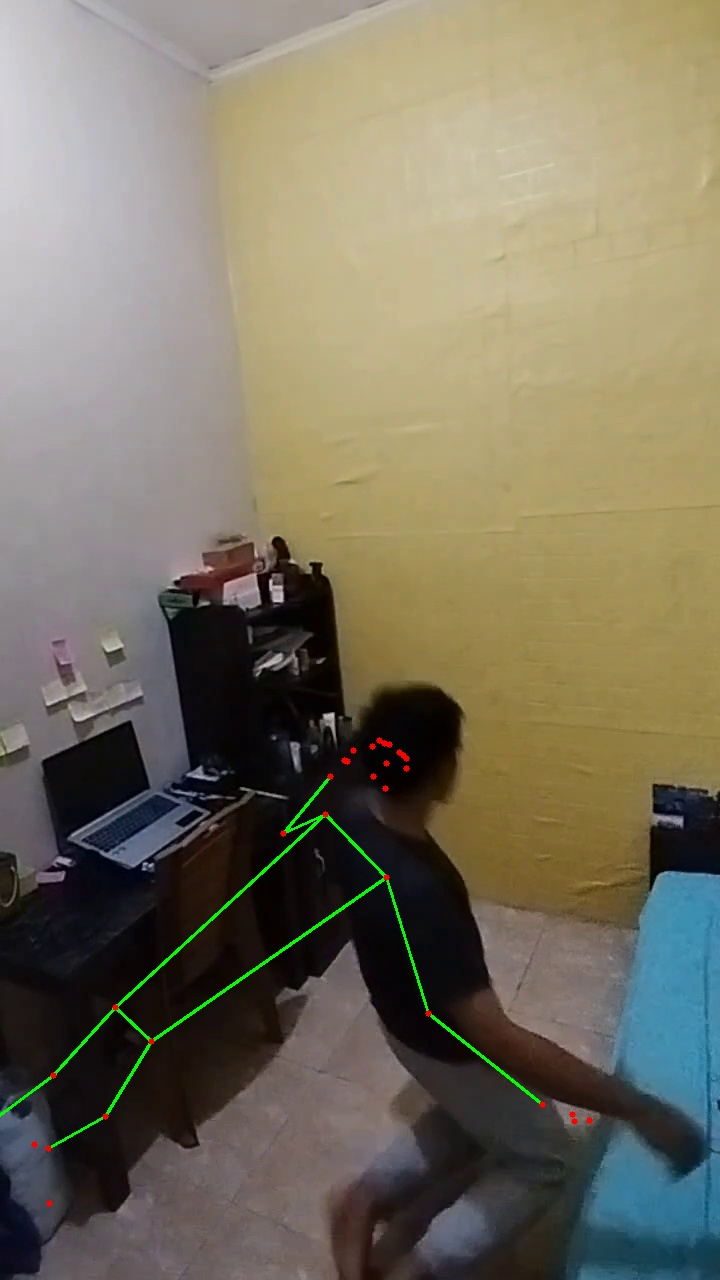
\includegraphics[trim=0cm 0cm 0cm 18cm, clip, width=\linewidth,height=5.0cm,keepaspectratio]{images/fall/fall_1.jpg} &
    tidak jatuh &
    jatuh \\
    \hline

    % ----- Row 2 -----
    2. &
    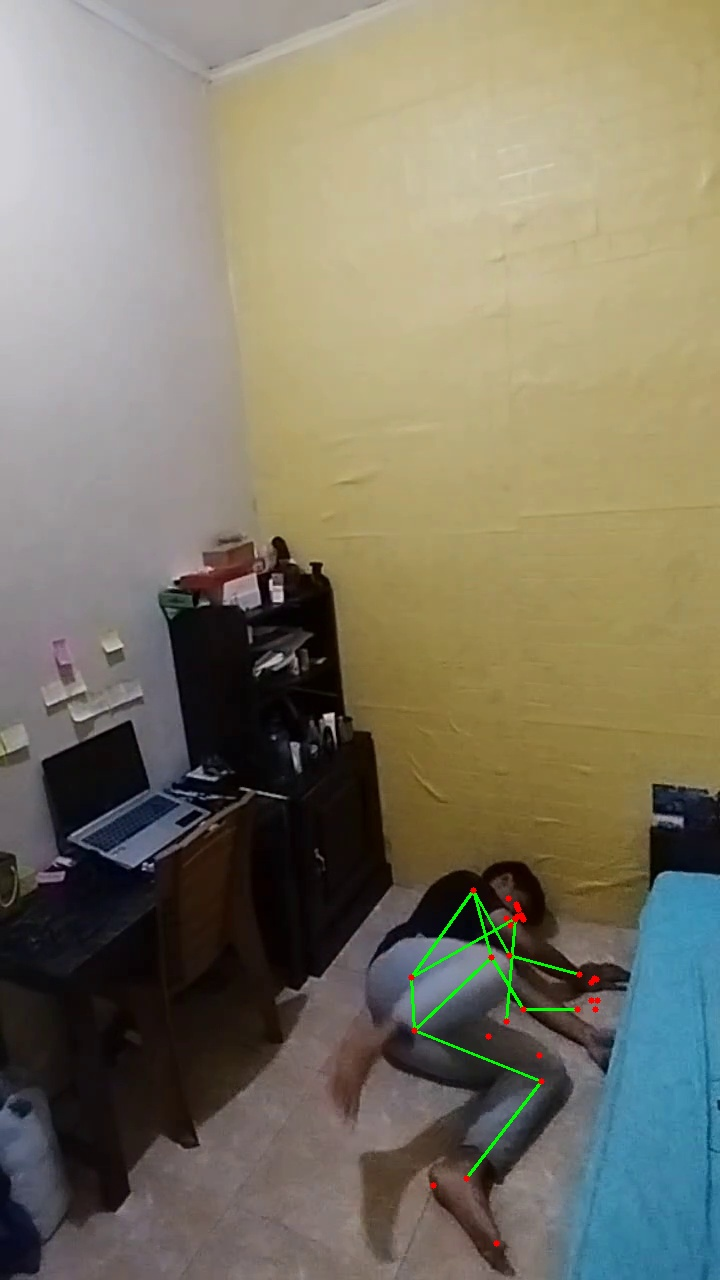
\includegraphics[trim=0cm 0cm 0cm 18cm, clip, width=\linewidth,height=5.0cm,keepaspectratio]{images/fall/fall_2.jpg} &
    jatuh &
    jatuh \\
    \hline

    % ----- Row 3 -----
    3. &
    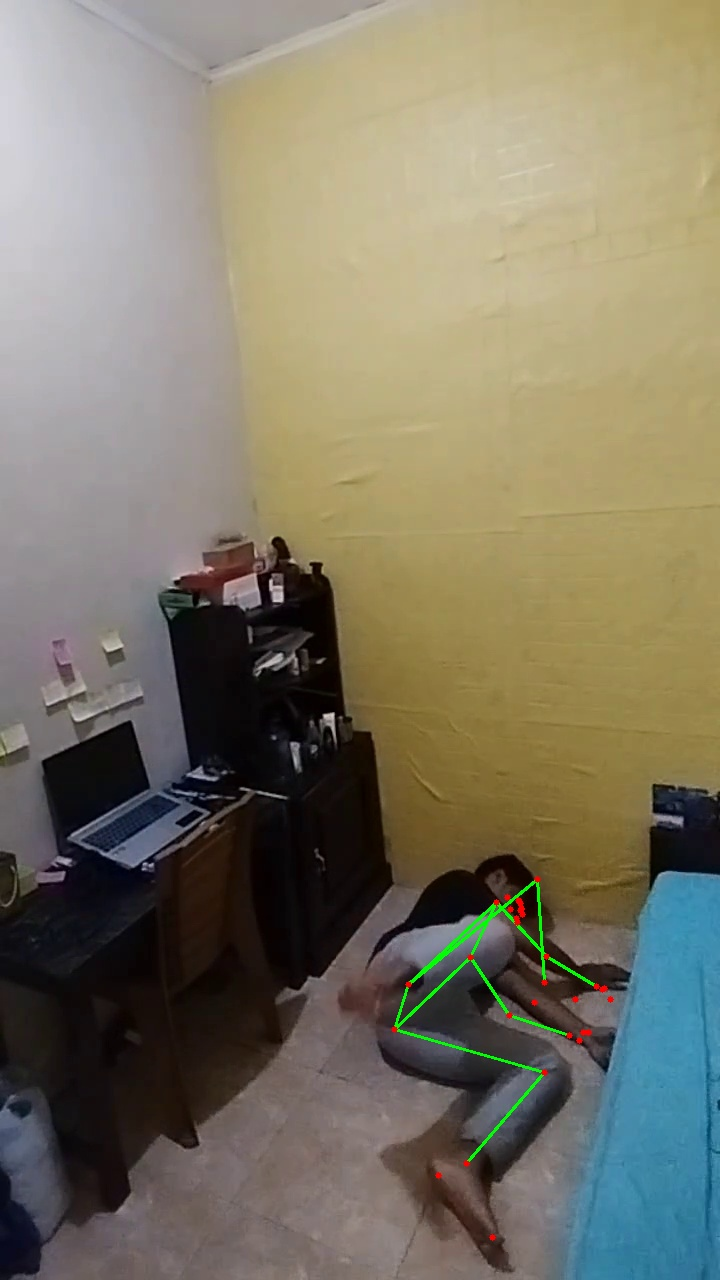
\includegraphics[trim=0cm 0cm 0cm 18cm, clip, width=\linewidth,height=5.0cm,keepaspectratio]{images/fall/fall_3.jpg} &
    jatuh &
    jatuh \\
    \hline

    % ----- Row 4 -----
    4. &
    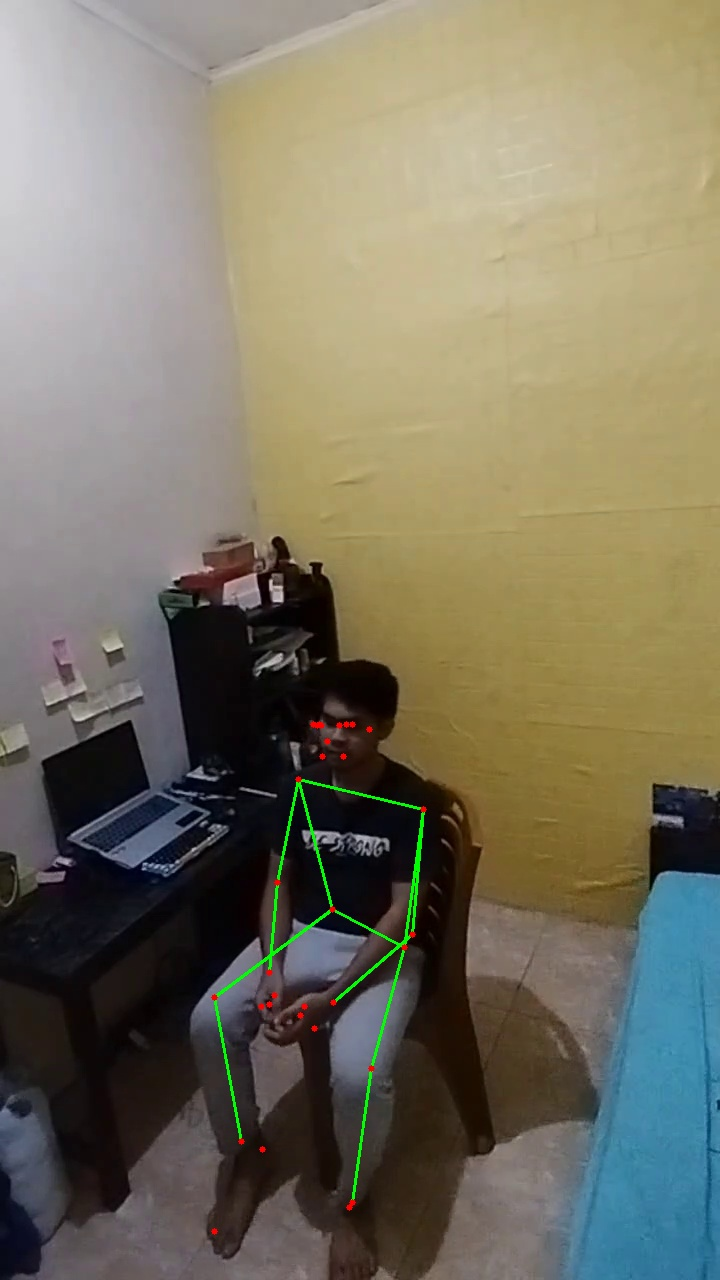
\includegraphics[trim=0cm 0cm 0cm 18cm, clip, width=\linewidth,height=5.0cm,keepaspectratio]{images/not_fall/not_fall_0.jpg} &
    jatuh &
    tidak jatuh \\
    \hline

    % ----- Row 5 -----
    5. &
    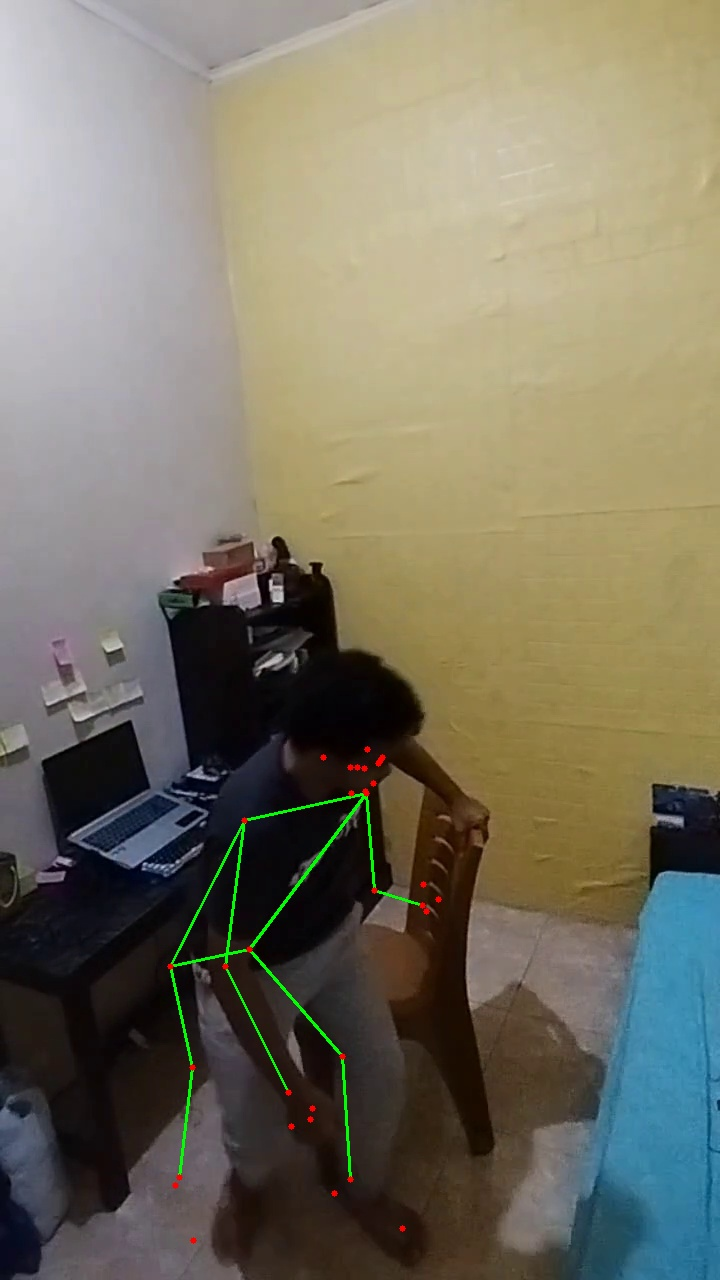
\includegraphics[trim=0cm 0cm 0cm 18cm, clip, width=\linewidth,height=5.0cm,keepaspectratio]{images/not_fall/not_fall_1.jpg} &
    jatuh &
    tidak jatuh \\
    \hline

    % ----- Row 6 -----
    6. &
    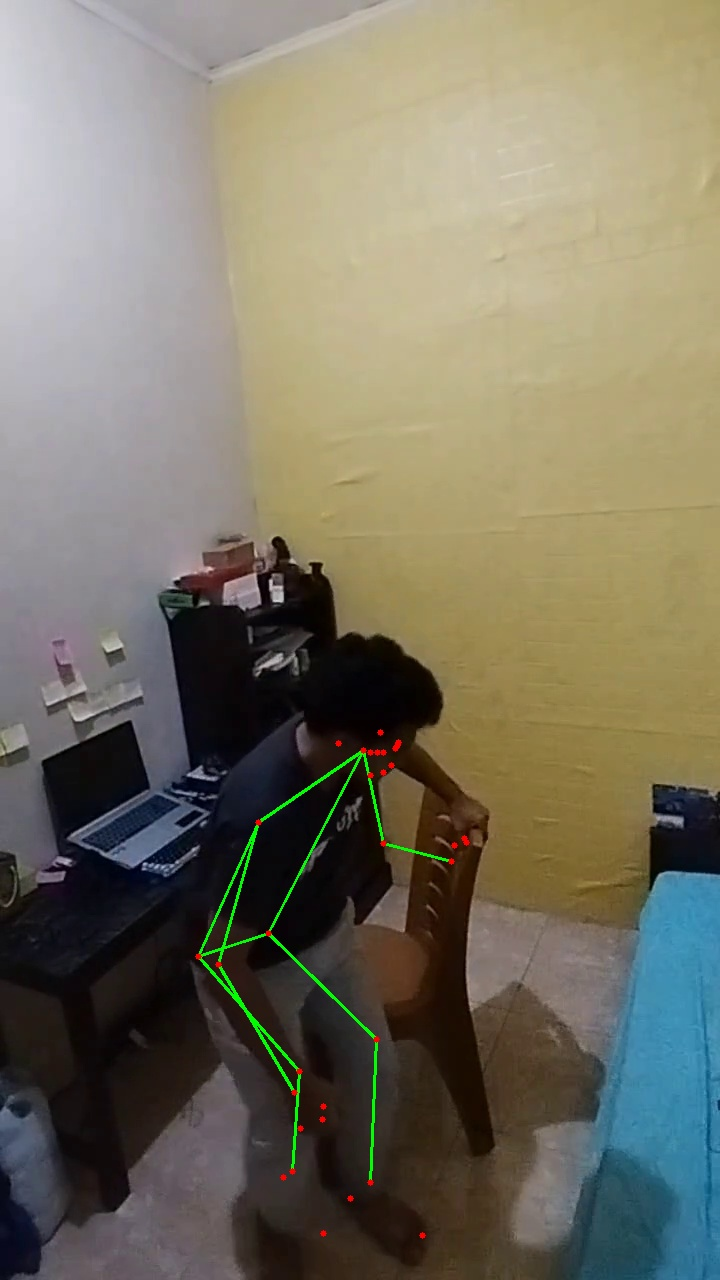
\includegraphics[trim=0cm 0cm 0cm 18cm, clip, width=\linewidth,height=5.0cm,keepaspectratio]{images/not_fall/not_fall_2.jpg} &
    jatuh &
    tidak jatuh \\
    \hline

\end{longtable}


\subsection{Evaluasi Studi Ablasi} \label{IV.evaluasi-ablasi}
Studi ablasi pada penelitian ini bertujuan untuk memahami kontribusi masing-masing \textit{hyperparameter} terhadap kinerja model \textit{Graph Convolutional Network} (GCN) dalam tugas deteksi posisi jatuh berbasis \textit{pose landmark} pada lansia. Lima \textit{hyperparameter} yang dievaluasi yaitu \textit{optimizer}, \textit{learning rate}, \textit{batch size}, \textit{weight decay}, dan \textit{dropout}. Pemilihan kelima faktor ini didasarkan pada pengaruh langsungnya terhadap stabilitas pelatihan, kemampuan generalisasi, serta efisiensi konvergensi pada arsitektur GCN. \par

Seluruh eksperimen dilakukan pada susunan data fold ke-4 karena pada pelatihan default konfigurasi ini memberi akurasi tertinggi. Dengan demikian, perbandingan menjadi adil karena hanya satu \textit{hyperparameter} diubah setiap kali (yang lain ditahan konstan). Setiap variasi dinilai terhadap \textit{baseline} menggunakan confusion matrix yang berfokus pada metrik akurasi. Tujuannya adalah mengidentifikasi \textit{hyperparameter} paling berpengaruh, sensitivitas model, serta merekomendasikan pengaturan optimal untuk eksperimen lanjutan dan implementasi akhir. \par

\subsubsection{\textit{Optimizer}} \label{IV.optimizer}
\begin{table}[htbp]
    \centering
    \caption{Hasil evaluasi studi ablasi optimizer}
    \label{tab:ablasi optimizer}
    \begin{tabular}{|c|c|c|c|c|c|c|c|c|}
        \hline
        \multirow{2}{*}{\textbf{Optimizer}} & \multicolumn{4}{c|}{\textbf{Hasil \textit{Confusion Matrix}}} & \multicolumn{4}{c|}{\textbf{Metrik Evaluasi}} \\ \cline{2-9}
         & \textbf{TP} & \textbf{TN} & \textbf{FP} & \textbf{FN} & \textbf{Acc} & \textbf{Pre} & \textbf{Rec} & \textbf{F1} \\ \hline
        AdamW & 1147 & 549 & 285 & 550 & 0.67 & 0.702 & 0.67 & 0.679 \\ \hline
        RMSProp & 1222  & 531 & 303 & 475 & \textbf{0.693} & 0.711 & 0.693 & 0.699 \\ \hline
        LION & 1158 & 523 & 311 & 539 & 0.664 & 0.691 & 0.664 & 0.672 \\ \hline
        % \multicolumn{5}{|c|}{\textit{Rata-rata}} & 0,665 & 0,694 & 0,59 & 0,638 \\ \hline
    \end{tabular}
\end{table}

Pada evaluasi optimizer yang terlihat pada Tabel \ref{tab:ablasi optimizer}, RMSProp memberikan kinerja terbaik dengan Acc 0,693, Pre 0,711, Rec 0,693, dan F1 0,699; ini tercermin dari TP tertinggi (1222) dan FN terendah (475), sehingga lebih banyak kejadian jatuh berhasil ditangkap meski spesifisitasnya moderat (~0,636). AdamW berada di posisi kedua (Acc 0,670; F1 0,679) dengan FP terendah (285) dan spesifisitas tertinggi (~0,658), artinya paling sedikit false alarm namun lebih banyak kejadian terlewat (FN 550, Rec 0,670). LION menghasilkan metrik terendah (Acc 0,664; F1 0,672) dengan FP dan FN sama-sama lebih tinggi (311 dan 539), menandakan konsistensi deteksi yang lebih lemah. Bedasarkan data tersebut, konfigurasi yang berfokus pada akurasi urutannya adalah RMSProp (0,693), kemudian AdamW (0,670), dan LION (0,664). RMSProp adalah pilihan terbaik, dengan AdamW sebagai alternatif kedua dan LION tidak direkomendasikan untuk konfigurasi ini.


\subsubsection{\textit{Learning Rate}} \label{IV.lr}

\begin{table}[htbp]
    \centering
    \caption{Hasil evaluasi studi ablasi learning rate}
    \label{tab:ablasi lr}
    \begin{tabular}{|c|c|c|c|c|c|c|c|c|}
        \hline
        \multirow{2}{*}{\textbf{Learning Rate}} & \multicolumn{4}{c|}{\textbf{Hasil \textit{Confusion Matrix}}} & \multicolumn{4}{c|}{\textbf{Metrik Evaluasi}} \\ \cline{2-9}
         & \textbf{TP} & \textbf{TN} & \textbf{FP} & \textbf{FN} & \textbf{Acc} & \textbf{Pre} & \textbf{Rec} & \textbf{F1} \\ \hline
        1e-2 & 1469 & 427 & 407 & 228 & \textbf{0.749} & 0.74 & 0.749 & 0.74 \\ \hline
        1e-3 & 1132  & 528 & 306 & 565 & 0.656 & 0.687 & 0.656 & 0.665 \\ \hline
        1e-4 & 1045 & 569 & 265 & 652 & 0.638 & 0.688 & 0.638 & 0.649 \\ \hline
        % \multicolumn{5}{|c|}{\textit{Rata-rata}} & 0,665 & 0,694 & 0,59 & 0,638 \\ \hline
    \end{tabular}
\end{table}

pada tabel \ref{tab:ablasi lr} terlihat studi learning rate yang menunjukkan nilai 0,01 menghasilkan kinerja paling kuat di seluruh metrik utama, dengan nilai Acc 0,749, Pre 0,740, Rec 0,749, F1 0,740, didorong oleh TP tertinggi (1469) dan FN terendah (228) sehingga lebih banyak kejadian jatuh terdeteksi. Konsekuensinya, FP juga tertinggi (407) sehingga spesifisitas lebih rendah. Menurunkan laju belajar ke 0,001 menekan FP (306) dan menaikkan TN (528), namun FN melonjak (565) sehingga Acc turun ke 0,656 dan model menjadi lebih “hati-hati” namun sering melewatkan kejadian. Dengan 0,0001, tren ini makin kuat: FP terendah (265) dan TN tertinggi (569) menunjukkan spesifisitas terbaik, tetapi FN meningkat tajam (652) sehingga Rec dan Acc melemah (0,638). Urutan nilai learning rate berdasarka akurasi adalah 0,01 (0,749), 0,001 (0,656), 0,0001 (0,638). \par

\subsubsection{\textit{Batch Size}} \label{IV.batch_size}

\begin{table}[htbp]
    \centering
    \caption{Hasil evaluasi studi ablasi batch size}
    \label{tab:ablasi batch size}
    \begin{tabular}{|c|c|c|c|c|c|c|c|c|}
        \hline
        \multirow{2}{*}{\textbf{Batch Size}} & \multicolumn{4}{c|}{\textbf{Hasil \textit{Confusion Matrix}}} & \multicolumn{4}{c|}{\textbf{Metrik Evaluasi}} \\ \cline{2-9}
         & \textbf{TP} & \textbf{TN} & \textbf{FP} & \textbf{FN} & \textbf{Acc} & \textbf{Pre} & \textbf{Rec} & \textbf{F1} \\ \hline
        16 & 1149 & 531 & 303 & 548 & 0.664 & 0.693 & 0.664 & 0.672 \\ \hline
        32 & 1105  & 560 & 274 & 592 & 0.658 & 0.697 & 0.658 & 0.668 \\ \hline
        64 & 1218 & 521 & 313 & 479 & \textbf{0.687} & 0.705 & 0.687 & 0.693 \\ \hline
        % \multicolumn{5}{|c|}{\textit{Rata-rata}} & 0,665 & 0,694 & 0,59 & 0,638 \\ \hline
    \end{tabular}
\end{table}

Pada uji batch size dalam tabel \ref{tab:ablasi batch size}, performa paling stabil justru muncul saat ukuran batch diperbesar. Batch 64 mencatat TP tertinggi (1218) dan FN terendah (479), sehingga recall dan F1 ikut naik (0,687 dan 0,693). Konsekuensinya, FP sedikit naik (313) dan TN turun (521). Batch 16 memberi hasil menengah (Acc 0,664) dengan FP 303 dan FN 548. Sementara batch 32 terlihat paling “konservatif” terhadap \textit{false alarm} (FP terendah 274, TN tertinggi 560), dikuti dengan TP terendah (1105) dan FN tertinggi (592), sehingga recall dan akurasinya ikut turun. Urutan nilai Batch size berdasarkan akurasi adalah batch 64 (0,687), batch 16 (0,664), batch 32 (0,658), sehingga dalam memaksimalkan akurasi pada konfigurasi ini, batch size 64 adalah pilihan terbaik. \par

\subsubsection{\textit{Weight Decay}} \label{IV.weight-decay}

\begin{table}[htbp]
    \centering
    \caption{Hasil evaluasi studi ablasi Weight Decay}
    \label{tab:ablasi Weight Decay}
    \begin{tabular}{|c|c|c|c|c|c|c|c|c|}
        \hline
        \multirow{2}{*}{\textbf{Weight Decay}} & \multicolumn{4}{c|}{\textbf{Hasil \textit{Confusion Matrix}}} & \multicolumn{4}{c|}{\textbf{Metrik Evaluasi}} \\ \cline{2-9}
         & \textbf{TP} & \textbf{TN} & \textbf{FP} & \textbf{FN} & \textbf{Acc} & \textbf{Pre} & \textbf{Rec} & \textbf{F1} \\ \hline
        1e-4 & 1300 & 508 & 326 & 397 & 0.714 & 0.721 & 0.714 & 0.717 \\ \hline
        1e-5 & 1344 & 483 & 351 & 353 & 0.722 & 0.722 & 0.722 & 0.722 \\ \hline
        1e-6 & 1321 & 511 & 323 & 376 & \textbf{0.724} & 0.729 & 0.724 & 0.726 \\ \hline
        % \multicolumn{5}{|c|}{\textit{Rata-rata}} & 0,665 & 0,694 & 0,59 & 0,638 \\ \hline
    \end{tabular}
\end{table}

Pada studi weight decay dalam tabel \ref{tab:ablasi Weight Decay}, penurunan laju regularisasi memberi pola yang cukup konsisten. Nilai 0,000001 menghasilkan kinerja paling seimbang dengan Acc 0,724, Pre 0,729, Rec 0,724, dan F1 0,726; kombinasi TP 1321 / FN 376 menunjukkan deteksi kejadian jatuh yang baik tanpa terlalu banyak \textit{false alarm} (FP 323, TN 511). Sedikit lebih besar, 0,00001 mendorong TP tertinggi (1344) dan FN terendah (353) sehingga recall naik, tetapi diimbangi oleh FP tertinggi (351) dan TN terendah (483) yang menekan spesifisitas; akurasinya berada di tengah (0,722). Sementara 0,0001 membuat keseimbangan membaik di sisi FP/TN (326/508), namun FN meningkat (397) sehingga akurasi turun (0,714). Urutan nilai \textit{weight decay} berdasarkan akurasi adalah 1e-6 (0,724), 1e-5 (0,722), 1e-6 (0,714). Demi memaksimalkan akurasi pada konfigurasi ini, weight decay 1e-6 adalah pilihan terbaik. \par

\subsubsection{\textit{Dropout}} \label{IV.dropout}

\begin{table}[htbp]
    \centering
    \caption{Hasil evaluasi studi ablasi Dropout}
    \label{tab:ablasi Dropout}
    \begin{tabular}{|c|c|c|c|c|c|c|c|c|}
        \hline
        \multirow{2}{*}{\textbf{Dropout}} & \multicolumn{4}{c|}{\textbf{Hasil \textit{Confusion Matrix}}} & \multicolumn{4}{c|}{\textbf{Metrik Evaluasi}} \\ \cline{2-9}
         & \textbf{TP} & \textbf{TN} & \textbf{FP} & \textbf{FN} & \textbf{Acc} & \textbf{Pre} & \textbf{Rec} & \textbf{F1} \\ \hline
        0,2 & 1178 & 557 & 277 & 519 & \textbf{0.686} & 0.713 & 0.686 & 0.693 \\ \hline
        0,3 & 1138  & 521 & 313 & 559 & 0.656 & 0.685 & 0.656 & 0.664 \\ \hline
        0,4 & 1102 & 559 & 275 & 595 & 0.656 & 0.696 & 0.656 & 0.666 \\ \hline
        % \multicolumn{5}{|c|}{\textit{Rata-rata}} & 0,665 & 0,694 & 0,59 & 0,638 \\ \hline
    \end{tabular}
\end{table}

Pada studi dropout dalam tabel \ref{tab:ablasi Dropout}, tingkat 0,2 memberi keseimbangan terbaik dengan metrik evaluasi Acc 0,686 (tertinggi), Pre 0,713, Rec 0,686, F1 0,693, ditopang TP 1178 dan FN 519 sehingga lebih banyak kejadian jatuh tertangkap dengan kenaikan \textit{false alarm} yang relatif kecil (FP 277). Menaikkan dropout ke 0,3 menurunkan kinerja di hampir semua metrik (Acc 0,656, F1 0,664) dengan FN meningkat (559) dan FP juga tinggi (313). Pada 0,4, presisi sedikit membaik (0,696) dan \textit{false alarm} paling rendah (FP 275, TN 559), tetapi banyak kejadian terlewat (FN 595), sehingga recall dan F1 turun. berdasarkan data tersebut dapat disimpulkan bahwa dropout 0,2 menghasilkan akurasi tertinggi (0,686), sedangkan 0,3 dan 0,4 setara di 0,656. jika fokus pada akurasi saja, nilai 0,2 adalah pilihan terbaik, dengan 0,4 hanya dipertimbangkan bila prioritasnya meminimalkan \textit{false alarm}.

% \subsubsection{Analisis pengaruh hyperparamter pada studi ablasi} \label{IV.model-ablasi}

\section{Perbandingan Hasil \textit{Hyperparameter} Default dengan Studi Ablasi} \label{IV.Analisis}


\begin{table}[htbp]
    \centering
    \caption{Perbandingan Konfigurasi \textit{hyperparameter} Default dan hasil Studi Ablasi}
    \label{tab:hyperparams-default-ablasi}
    \begin{tabular}{|c|c|c|c|}
        \hline
        \textbf{No} & \textbf{\textit{Hyperparameter}} & \textbf{Default} & \textbf{Studi Ablasi} \\ \hline
        1 & \textit{optimizers}          & AdamW & RMSProp\\ \hline        
        2 & \textit{learning rate}     & 1e-3 & 1e-2 \\ \hline
        3 & \textit{batch size}        & 32 & 64 \\ \hline
        4 & \textit{weight decay}      & 1e-5 & 1e-6 \\ \hline
        5 & \textit{dropout rate}      & 0.3 & 0,2 \\ \hline
        6 & \textit{hidden\_channels}    & [64, 32, 32, 32, 32] & [64, 32, 32, 32, 32] \\ \hline
        7 & \textit{epochs}              & 100 & 100 \\ \hline
        8 & \textit{residuals}           & \textit{True} & \textit{True} \\ \hline
    \end{tabular}
\end{table}

Tabel \ref{tab:hyperparams-default-ablasi} diperlihatkan perbedaan antara konfigurasi default dan hasil studi ablasi untuk model GCN deteksi jatuh berbasis pose landmark. Perubahan utamanya berada di sisi optimisasi dan regularisasi, optimizer bergeser dari AdamW ke RMSProp yang pada eksperimen memberi konvergensi lebih stabil untuk data landmark, learning rate dinaikkan dari 1e-3 ke 1e-2 agar langkah pembaruan bobot lebih cepat, batch size diperbesar dari 32 ke 64 untuk menurunkan noise gradien, weight decay diturunkan dari 1e-5 ke 1e-6 guna mengurangi penalti berlebih pada bobot, dan dropout diturunkan dari 0,3 ke 0,2 agar kapasitas representasi tidak terlalu ditekan. Hasil Pelatihan ulang model menggunakan konfigurasi hyperparameter hasil studi ablasi dapat dilihat pada tabel \ref{tab:evaluasi-fold-ablasi}.


\begin{table}[htbp]
    \centering
    \caption{Hasil evaluasi studi ablasi per fold dan rerata}
    \label{tab:evaluasi-fold-ablasi}
    \begin{tabular}{|c|c|c|c|c|c|c|c|c|}
        \hline
        \multirow{2}{*}{\textbf{Fold}} & \multicolumn{4}{c|}{\textbf{Hasil \textit{Confusion Matrix}}} & \multicolumn{4}{c|}{\textbf{Metrik Evaluasi}} \\ \cline{2-9}
         & \textbf{TP} & \textbf{TN} & \textbf{FP} & \textbf{FN} & \textbf{Acc} & \textbf{Pre} & \textbf{Rec} & \textbf{F1} \\ \hline
        1 & 458 & 1378 & 319 & 376 & \textbf{0,725} & 0,721 & \textbf{0,725} & \textbf{0,723} \\ \hline
        2 & 677 & 216 & 59 & 397 & 0,662 & \textbf{0,804} & 0,662 & 0,695 \\ \hline
        3 & 410 & 1181 & 283 & 467 & 0,68 & 0,67 & 0,68 & 0,67 \\ \hline
        4 & 719 & 410 & 147 & 302 & 0,716 & 0,741 & 0,716 & 0,721 \\ \hline
        5 & 500  & 573 & 184 & 444 & 0,631 & 0,656 & 0,631 & 0,628 \\ \hline
        \multicolumn{5}{|c|}{\textit{Rata-rata}} & 0,683 & 0,718 & 0,683 & 0,687 \\ \hline
    \end{tabular}
\end{table}

Tabel \ref{tab:evaluasi-fold-ablasi} menunjukkan hasil kinerja model klasifikasi jatuh dan tidak jatuh pada skema 5-fold menggunakan kombinasi hyperparameter terbaik hasil studi ablasi. Secara umum, performa berada di rentang akurasi 0,631–0,725 dengan rerata 0,683. Rata-rata precision 0,718 lebih tinggi daripada recall 0,683, sehingga F1 rata-rata mencapai 0,687. Fold 1 tampil paling kuat dengan akurasi 0,725 dan recall 0,725 (F1 0,723), ditopang TP yang relatif tinggi (458) meski FP masih ada (319). Fold 4 juga stabil (Acc 0,716, F1 0,721) dengan keseimbangan FP/FN yang lebih baik (147/302). Sebaliknya, Fold 2 menunjukkan precision tertinggi 0,804 karena FP sangat rendah (59), namun banyak kasus positif terlewat (FN 397), sehingga akurasinya tidak menjadi yang terbaik (0,662). Fold 5 terendah (Acc 0,631), ditandai FN yang tinggi (444). Pola precision yang lebih besar dari recall konsisten di sebagian besar fold, menandakan model cenderung lebih jarang memberi alarm palsu, tetapi masih melewatkan sebagian kejadian jatuh, kemungkinan dipengaruhi variasi distribusi sampel antar fold akibat pembagian berbasis folder. \par

\begin{table}[htbp]
    \centering
    \caption{Perbandingan hasil evaluasi per fold konfigurasi default dan studi ablasi}
    \label{tab:perbandingan cm default ablasi}
    \begin{tabular}{|c|c|c|c|c|c|c|c|c|c|}
        \hline
        \multirow{2}{*}{\textbf{Fold}} & \multirow{2}{*}{\textbf{Konfigurasi}} & \multicolumn{4}{c|}{\textbf{Hasil \textit{Confusion Matrix}}} & \multicolumn{4}{c|}{\textbf{Metrik Evaluasi}} \\ \cline{3-10}
         & & \textbf{TP} & \textbf{TN} & \textbf{FP} & \textbf{FN} & \textbf{Acc} & \textbf{Pre} & \textbf{Rec} & \textbf{F1} \\ \hline
        1 & default & 558 & 1105 & 592 & 276 & 0,657 & 0,696 & 0,657 & 0,667 \\ \cline{2-10}
         & Ablasi & 458 & \textbf{1378} & 319 & 376 & \textbf{0,725} & 0,721 & \textbf{0,725} & \textbf{0,723} \\ \hline
        2 & default & 613 & 232 & 43 & 461 & 0,626 & \textbf{0,812} & 0,626 & 0,662 \\ \cline{2-10}
         & Ablasi & 677 & 216 & 59 & 397 & 0,662 & 0,804 & 0,662 & 0,695 \\ \hline
        3 & default & 425 & 1165 & 299 & 452 & 0,679 & 0,671 & 0,679 & 0,672 \\ \cline{2-10}
         & Ablasi & 410 & 1181 & 283 & 467 & 0,68 & 0,67 & 0,68 & 0,67 \\ \hline
        4 & default & 703 & 419 & 138 & 318 & 0,711 & 0,742 & 0,711 & 0,717 \\ \cline{2-10}
         & Ablasi & \textbf{719} & 410 & 147 & 302 & 0,716 & 0,741 & 0,716 & 0,721 \\ \hline
        5 & default & 501 & 594 & 163 & 443 & 0,644 & 0,674 & 0,644 & 0,641 \\ \cline{2-10}
         & Ablasi & 500  & 573 & 184 & 444 & 0,631 & 0,656 & 0,631 & 0,628 \\ \hline
    \end{tabular}
\end{table}

Berdasarkan Tabel \ref{tab:perbandingan cm default ablasi}, pengaruh perubahan konfigurasi hyperparameter dari konfigurasi \textit{default} ke hasil studi ablasi menunjukkan pola peningkatan performa yang tidak simetris antara kelas jatuh dan tidak jatuh. Analisis difokuskan pada komponen \textit{confusion matrix}, terutama nilai \textit{True Positive} (TP) yang merepresentasikan kemampuan model dalam mendeteksi posisi jatuh, serta \textit{True Negative} (TN) yang menunjukkan ketepatan model memprediksi posisi tidak jatuh. \par

Pada fold-1, penerapan \textit{hyperparameter} hasil studi ablasi menghasilkan peningkatan TN yang sangat signifikan, meningkat sebesar 223 prediksi benar pada kelas tidak jatuh. Peningkatan ini sejalan dengan kenaikan nilai akurasi sebesar 0,068, recall sebesar 0,068, serta skor F1 sebesar 0,056, yang mengindikasikan bahwa konfigurasi ablasi meningkatkan kemampuan generalisasi model dalam menghindari kesalahan klasifikasi posisi tidak jatuh sebagai posisi jatuh. \par

Pada fold-2 dan fold-4, peningkatan performa justru lebih dominan pada kelas jatuh, yang ditunjukkan oleh kenaikan TP masing-masing sebesar 64 (dari 613 menjadi 677) dan 16 (dari 703 menjadi 719). Namun demikian, peningkatan tersebut tidak diikuti oleh lonjakan metrik evaluasi secara keseluruhan, khususnya akurasi dan F1-score, yang relatif stabil dibandingkan fold-1. Pada fold-3, peningkatan TN hanya sebesar 16, sedangkan pada fold-5 konfigurasi default masih sedikit lebih unggul dibandingkan konfigurasi ablasi, baik dari sisi TP maupun TN, yang menunjukkan bahwa efek ablasi tidak selalu konsisten pada seluruh pembagian data. \par

Secara keseluruhan, meskipun studi ablasi terlihat mampu meningkatkan kemampuan deteksi posisi jatuh pada beberapa fold, peningkatan performa yang paling signifikan justru terjadi pada kelas tidak jatuh (TN), terutama pada fold-1 yang menunjukkan selisih prediksi benar terbesar. Hal ini mengindikasikan bahwa konfigurasi \textit{hyperparameter} hasil studi ablasi lebih efektif dalam menekan \textit{false alarm} atau kesalahan positif palsu, sehingga meningkatkan stabilitas model dalam mengenali aktivitas tidak jatuh. Berdasarkan hal ini, didapatkan bahwa peningkatan performa setelah studi ablasi cenderung lebih signifikan pada kelas tidak jatuh. \par

% Perubahan peforma pelatihan model antara menggunakan konfigurasi default dan studi ablasi secara detail dapat dilihat pada Tabel \ref{tab:perbandingan cm default ablasi}.Fokus pada hasil confusion matrix, pada fold-1, konfigurasi studi ablasi memberikan peningkatan peforma model dengan improvement prediksi tepat pada kelas tidak jatuh (TN) sebesar 223 dari konfigurasi default. Kemudian pada fold-2, terdapat peningkatan peforma model pada kelas jatuh (TP) menggunakan ablasi sebesar 64. Lalu pada Fold-3 terdapat peningkatan prediksi terhadap TN sebesar 16. Pada Fold-4 terdapat peningkatan prediksi TP sebesar 16 juga. Namun pada Fold-5, peforma model pada konfigurasi default masih sedikit lebih unggul terhadap konfigurasi ablasi. Akan tetapi, melihat perbedaan peforma terbesar yang ada pada fold-1 mengindikasikann bahwa konfigurasi hyperparameter menggunakan studi ablasi memberikan peningkatan pelatihan model secara signifikan terhadap kelas tidak jatuh (TN).

\begin{table}[htbp]
    \centering
    \caption{Perbandingan Hasil evaluasi konfigurasi hyperparamter default dan studi ablasi}
    \label{tab:perbandingan hasil hyperparameter default dan studi ablasi}
    \begin{tabular}{|c|c|c|c|c|}
        \hline
        \multirow{2}{*}{\textbf{konfigurasi \textit{hyperparameter}}} & \multicolumn{4}{c|}{\textbf{Rerata Metrik Evaluasi}} \\ \cline{2-5}
         & \textbf{Acc} & \textbf{Pre} & \textbf{Rec} & \textbf{F1} \\ \hline
        Default & 0,665 & 0,694 & 0,59 & 0,638 \\ \hline
        Studi ablasi & \textbf{0,683} & \textbf{0,718} & \textbf{0,683} & \textbf{0,687} \\ \hline
    \end{tabular}
\end{table}

Tabel \ref{tab:perbandingan hasil hyperparameter default dan studi ablasi} membandingkan rerata metrik 5-fold antara konfigurasi default dan konfigurasi hasil studi ablasi (nilai terbaik per hyperparameter). Secara keseluruhan, kombinasi dari studi ablasi memberikan dorongan kinerja yang konsisten, akurasi naik dari 0,665 → 0,683 (peningkatan sebesar 0,018), presisi dari 0,694 → 0,718 (peningkatan sebesar 0,024), dan F1 dari 0,638 → 0,687 (peningkatan sebesar 0,049). Peningkatan terbesar terlihat pada recall, dari 0,590 → 0,683 (peningkatan sebesar 0,093), yang berarti model sedikit lebih jarang meloloskan kejadian jatuh (miss) dibanding konfigurasi awal. Karena presisi juga ikut naik, perbaikan ini tidak “dibayar” dengan lonjakan false alarm, justru prediksi positif menjadi lebih tepat sekaligus lebih lengkap. Dengan kata lain, \textit{hyperparameter} hasil studi ablasi membuat model lebih andal di dua sisi, lebih akurat secara agregat dan lebih sensitif menangkap kejadian jatuh, tanpa mengorbankan ketepatan prediksi positif. Visualisasi perbedaan antara kedua konfigurasi tersebut ditampilkan pada Gambar \ref{fig:chart perbedaan default ablasi} untuk melihat seberapa jauh peningkatan peforma model.

\begin{figure}[htbp]  % 'h' menunjukkan gambar akan diletakkan di sekitar posisi ini
    \centering  % Gambar dipusatkan
    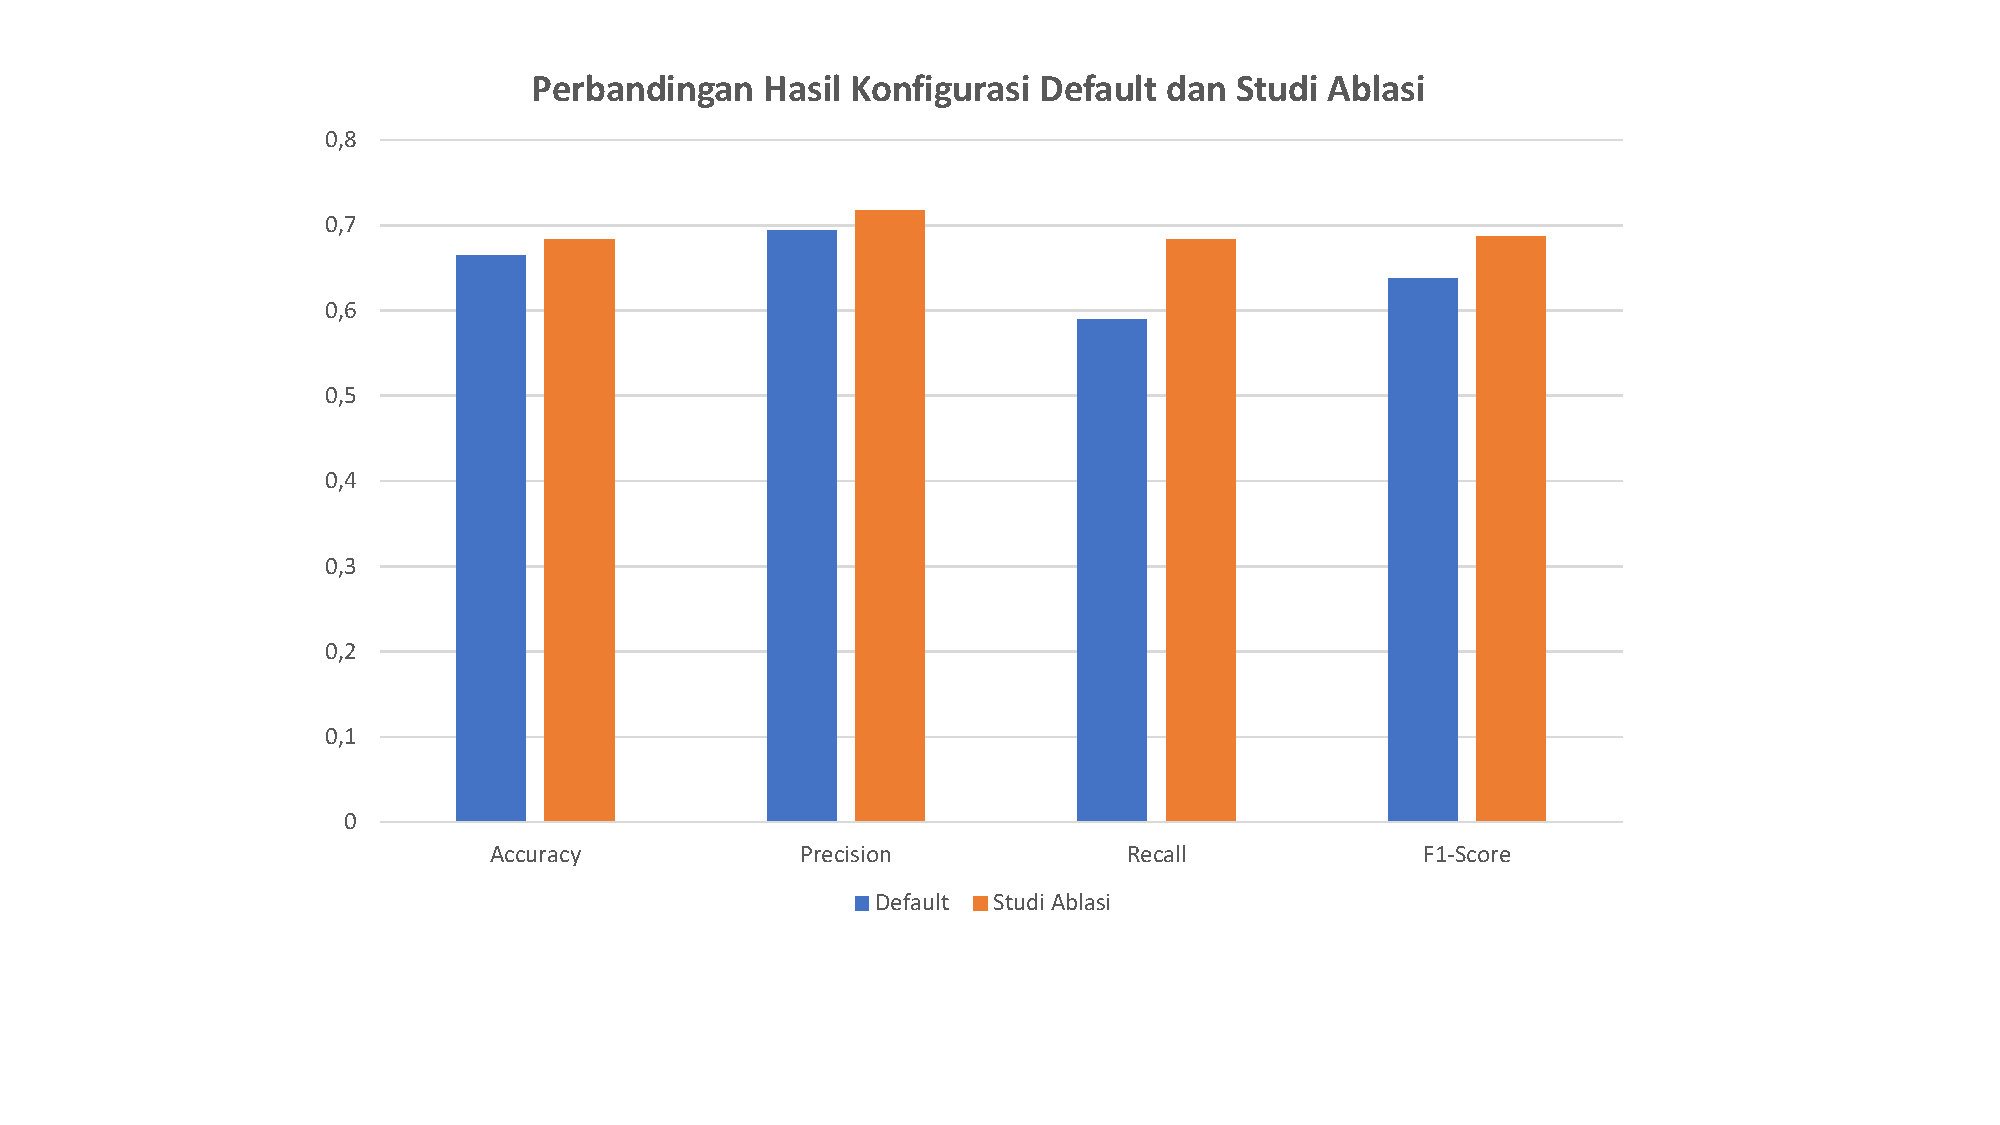
\includegraphics[width=1\textwidth]{figure/BAB 4/chart perbedaan konfigurasi default dan ablasi.pdf}  % Menyisipkan gambar dengan lebar setengah lebar teks
    \caption{Visualisasi perbedaan hasil pelatihan antara konfigurasi default dan studi ablasi}  % Menambahkan keterangan gambar
    \label{fig:chart perbedaan default ablasi}  % Menambahkan label untuk referensi
\end{figure}

Kinerja model pada konfigurasi \textit{hyperparameter} default maupun hasil studi ablasi masih berada di bawah capaian penelitian terdahulu, misalnya Zhang et al. (2023) yang melaporkan akurasi sebesar 96,3\% pada dataset MCF \cite{Zhang2023}. Namun, dalam perbandingan ini terdapat perbedaan mendasar yang perlu diperhatikan, baik pada arsitektur model maupun karakteristik data yang digunakan. Zhang et al. mengadopsi \textit{Dense Spatial-Temporal Graph Convolutional Network} yang secara eksplisit mengambil hubungan spasial dan temporal antar frame berurutan, sehingga memiliki kapasitas representasi fitur yang lebih tinggi untuk mengenali pola jatuh yang kompleks. Sebaliknya, penelitian ini secara sengaja membatasi penggunaan arsitektur \textit{Graph Convolutional Network} tanpa pemodelan spasial-temporal eksplisit dan hanya memanfaatkan representasi \textit{skeleton} dari \textit{Mediapipe Pose}. Pendekatan ini bertujuan untuk mengevaluasi sejauh mana model GCN yang lebih sederhana tetap mampu membangun diskriminasi kelas jatuh dan tidak jatuh. Oleh karena itu, capaian kinerja yang lebih rendah menjelaskan konsekuensi logis dari batasan arsitektural yang diterapkan, sekaligus menegaskan posisi penelitian ini sebagai studi evaluatif terhadap efisiensi dan kemampuan dasar GCN berbasis \textit{skeleton}. \par


\section{Rangkuman Hasil Keseluruhan} \label{IV.Bahas}
Dataset yang digunakan berupa rekaman video aktivitas manusia dari kamera 2D untuk mendokumentasikan skenario jatuh pada lingkungan realistis. Proses \textit{resampling} berdasarkan file \textit{metadata} menghasilkan 267 video jatuh dan 270 video tidak jatuh. Pada tahap prapemrosesan, diekstraksi total 16.110 citra dari seluruh video, kemudian dilakukan deteksi 33 \textit{pose landmark} menggunakan \textit{Mediapipe Pose}. Total data selanjutnya diseimbangkan antara kelas jatuh dan tidak jatuh hingga diperoleh total 9.500 data. Seluruh \textit{landmark} kemudian dikonversi menjadi representasi graf untuk memodelkan hubungan spasial antartitik tubuh secara terstruktur. Untuk mencegah kebocoran data, diterapkan skema \textit{5-fold}. \par

Perancangan arsitektur \textit{Graph Convolutional Network} (GCN) dapat dilihat pada Kode \ref{kode:inisialisasi gcn}. Model terdiri dari beberapa lapis \textit{GCNConv} yang diikuti \textit{BatchNorm1d}, aktivasi ReLU, serta \textit{dropout} untuk regularisasi. Opsi \textit{residual connection} diaktifkan secara kondisional ketika dimensi fitur kompatibel agar aliran gradien lebih stabil pada jaringan yang lebih dalam. Setelah tumpukan konvolusi graf, fitur node diagregasi menjadi representasi tingkat-graf melalui \textit{global pooling}, lalu dipetakan ke ruang keluaran menggunakan MLP dua lapis. Karena tugasnya klasifikasi biner, keluaran menggunakan aktivasi \textit{sigmoid} dengan satu neuron. \par

Pelatihan dilakukan menggunakan konfigurasi \textit{hyperparameter} default dan konfigurasi hasil studi ablasi. Pada konfigurasi default, pelatihan dijalankan selama 100 \textit{epoch} dengan \textit{batch size} 32, optimizer AdamW, \textit{learning rate} \(1\times 10^{-3}\), dan \textit{weight decay} \(1\times 10^{-5}\). Model menerima 3 fitur per node (\(x,y,z\)), menggunakan susunan \textit{hidden channels} \([64,32,32,32,32]\), \textit{dropout} 0,3, serta \textit{residual connection} aktif. Evaluasi \textit{5-fold} menunjukkan performa terbaik pada fold-4 dengan TP=703, FN=318, FP=138, dan TN=419, menghasilkan akurasi 0,711 dan F1 0,717. Secara umum, model cenderung memiliki presisi tinggi (lebih sedikit \textit{false alarm}), namun \textit{recall} lebih rendah. \par

Bobot terbaik dari pelatihan default berasal dari fold-4 pada epoch ke-2 dengan akurasi validasi 0,71 digunakan dalam tahap uji pada dataset primer. Pada pengujian, model mampu mengklasifikasikan 22 sampel jatuh dengan benar, tetapi masih cenderung memprediksi sebagian data tidak jatuh sebagai jatuh. Metrik pada data uji menunjukkan performa kurang memuaskan dengan akurasi 0,39, yang terutama dipengaruhi oleh karakteristik data uji kelas tidak jatuh yang berasal dari aktivitas duduk di kursi. \par

Studi ablasi dilakukan untuk menilai kontribusi lima \textit{hyperparameter}, yaitu \textit{optimizer}, \textit{learning rate}, \textit{batch size}, \textit{weight decay}, dan \textit{dropout}. Seluruh eksperimen dilakukan pada susunan data fold-4 agar perbandingan adil, dengan mengubah satu parameter dan menahan parameter lain tetap konstan. Hasil terbaik per parameter adalah RMSProp (akurasi 0,693), \textit{learning rate} 0,01 (0,749), \textit{batch size} 64 (0,687), \textit{weight decay} \(1\times 10^{-6}\) (0,724), dan \textit{dropout} 0,2 (0,686). Kombinasi terbaik kemudian dievaluasi kembali pada skema \textit{5-fold} dan menunjukkan fold-1 sebagai yang paling kuat (akurasi 0,725; \textit{recall} 0,725; F1 0,723). \par

Perbandingan \textit{confusion matrix} antara konfigurasi default dan hasil studi ablasi menunjukkan peningkatan performa yang tidak selalu konsisten pada seluruh fold. Peningkatan paling signifikan terjadi pada kelas tidak jatuh (kenaikan TN besar, terutama pada fold-1), yang mengindikasikan konfigurasi ablasi lebih efektif dalam menekan \textit{false alarm}. Meskipun beberapa fold menunjukkan kenaikan TP (kelas jatuh), dampaknya terhadap akurasi dan F1 tidak selalu besar. \par

Secara keseluruhan, konfigurasi hasil studi ablasi meningkatkan rerata kinerja model dibanding konfigurasi default, dengan peningkatan akurasi sebesar 0,018 (0,665 \(\rightarrow\) 0,683), presisi sebesar 0,024 (0,694 \(\rightarrow\) 0,718), F1-score sebesar 0,049 (0,638 \(\rightarrow\) 0,687), dan \textit{recall} sebesar 0,093 (0,590 \(\rightarrow\) 0,683). Meskipun demikian, kinerja model masih berada di bawah penelitian terdahulu seperti Zhang et al. (2023) yang melaporkan akurasi 96,3\% pada dataset MCF \cite{Zhang2023}. Perbedaan ini dipengaruhi oleh perbedaan dataset dan terutama arsitektur yang dikembangka Zhang et al. yang menggunakan \textit{Dense Spatial-Temporal Graph Convolutional Network} berfungsi memodelkan relasi spasial dan temporal antar \textit{frame} berurutan, sedangkan penelitian ini membatasi model pada GCN tanpa spasial-temporal eksplisit dan hanya memanfaatkan representasi \textit{skeleton} dari \textit{Mediapipe Pose} untuk mengevaluasi kemampuan dasar dan efisiensi pendekatan yang lebih sederhana. \par